\subsection*{Abstract}

Formal \ndx{specifications} are necessary to guarantee software meets critical
safety properties, but retrofitting \ndx{specifications} to existing software
requires considerable resources and expertise. Although inference eases
discovery of \ndx{specifications}, existing inference techniques are limited in
targeting different specification conditions. Particularly, inference of
\ndx{postcondition}s has rarely been the targeted focus of prior investigations.
This paper presents a static program analysis that automatically synthesizes
postconditions from pure program syntax. These postconditions represent final
values of variables in \ndx{numerical loops}. For each variable, the analysis
finds one approximative postcondition, of at most polynomial form, if it is
expressible in the underlying theory. This theory is a sound and compositional
flow calculus with complexity-theoretic origins. However, applying the flow
calculus to postcondition inference required several enhancements. As technical
contributions, we resolve multiple open problems about the flow calculus and
increase its expressive power. Experiments and comparison study show the
postcondition analysis is orthogonal to alternative techniques and generalizes
to classic algorithms. These findings suggest the \ndx{postcondition} analysis
can offer support in specification tasks even if full implementation details are
still in flux.

\subsection{Introduction}
\label{sec:pc-intro}

Software engineers have an aphorism that warns against publishing releases on
Fridays. It is shared lightheartedly, but embeds serious commentary about the
normalcy of software instability. Formal methods\index{formal methods} provides
the techniques to improve and achieve rigorous software quality guarantees.
Unfortunately, integrating formal methods to mainstream software development
workflows remains challenging due to, \eg lack of training and tool-specific
issues~\cite{beek2024}. Continued research effort must be dedicated to reducing
the entry barriers.

This paper aims to improve accessibility of formal methods. We do this by
introducing a program analysis that synthesizes partial specification
conditions. We develop an automatic inference of approximative
\ndx{postcondition}s in \ndx{numerical loops}. Postconditions are specialized
\ndx{assertion}s that must hold after the loop terminates.
They are complementary to inductive\index{invariant!inductive} loop\index{loop
invariant} \ndx{invariant}s, \ie conditions that must hold pre-iteration and be
preserved by the loop~\cite{sankaranarayanan2004}. Although postconditions may
be derivable from \ndx{invariant}s, loop\index{loop invariant} invariant
inference\index{invariant inference} is one of the hardest problems in
verification~\cite{dillig2013,si2018}. Therefore, we suggest the opposite
approach: starting with \ndx{postcondition}s. It is well-known that having
postconditions supports discovery of inductive\index{invariant!inductive}
\ndx{invariant}s~\cite{furia2010}\index{invariant!inductive}. Moreover, as
generalized \ndx{assertion}s, \ndx{postcondition}s assist
in various software development activities~\cite{nguyen2022}, like
testing\index{software testing}~\cite{alagarsamy2024,zhang2015} and code
maintenance~\cite{rosenblum1995}. However, dedicated studies of postcondition
inference are a novelty in research literature~\cite{popeea2006,molina2021}.

Specifications\index{specifications} must be precise, consistent, and complete
descriptions of program behavior. Making formal \ndx{specifications}
mechanically verifiable requires they are expressed in a structured language.
However, defining formal \ndx{specifications} is non-trivial and requires
expertise. In the meantime, various resource
analyses~\cite{jones2009,brockschmidt2016}\index{resource analysis} already
compute varied notions of \ndx{postcondition}s as means to arrive to their
primary result. Thus, it seems natural that {resource analyses could be used to
infer postconditions} for formal \ndx{specifications}. This is precisely the key
intuition we exploit in the paper. We present a complexity\hyp{}theoretic flow
calculus~\cite{jones2009,aubert20222}\index{mwp-calculus} that we use to
automatically infer variable \ndx{postcondition}s. In this view, the program
implements the intended behavior, but misses a formal proof. Our goal is to
assist software engineers in completing this missing step.

\subsubsection{Problem formulation and solution overview}
\label{subsec:overview}

We analyze deterministic imperative \ndx{numerical loops}. The loop may be
bounded or unbounded\index{unbounded loop}, with unknown \ndx{termination}
behavior. The loop manipulates a fixed number of natural number variables.
Beyond type, we make no assumptions about initial variable values. Our goal is
to automatically infer \ndx{postcondition}s of the variables occurring in the
loop. A postcondition is an \ndx{assertion} about a
variable's value that holds after iteration, if the loop terminates. The loop
may represent a program {fragment} that is still under development. Reducing
contextual information this way is practically motivated because such
information is commonly absent in realistic unverified programs.

\autoref{lst:exA} shows a canonical verification problem. Given a specification
with a \ndx{precondition} (\pr|assume|)\index{assumption} and a loop command
(\pr|for|), the goal of formal verification is to prove that the
\ndx{postcondition} (\pr|assert|\index{assertion}) is
satisfiable. The program \emph{\explain}, in \autoref{lst:exB}, shows the
problem variant we address in the paper. When precise variable values,
\ndx{precondition}, and iteration count are unknown, what postconditions
(\qtext) can we infer from the syntax?

\begin{center}
\begin{minipage}{.45\textwidth}
\captionsetup{type=lstlisting}
\begin{center}
\begin{minipage}{.9\textwidth}
\begin{implisting}*[numbers=none,escapeinside=||]
assume(X2|$\leq$|10|$\,\land\,$|X4==2|$\,\land\,$|X5>4);
for(i=0;i<10;i++) {
  X3=X2*X2;
  X3=X3+X5;
  X4=X4+X5; }
assert(X3|$\leq$|100+X5|$\,\land\,$|X4|$\geq$|42);
\end{implisting}
\end{minipage}
\end{center}
\captionof{lstlisting}[Precise context]
{Precise context (ideal).}\label{lst:exA}
\end{minipage}\hfill%
\begin{minipage}{.52\textwidth}
\captionsetup{type=lstlisting}
\begin{center}
\begin{minipage}{.85\textwidth}
\begin{implisting}*[numbers=none,escapeinside=||]
for(i=0;i<X1;i++) {
  X3=X2*X2;
  X3=X3+X5;
  X4=X4+X5; }
assert(|\myqm|);
\end{implisting}
\end{minipage}
\end{center}
\captionof{lstlisting}[Imprecise context]
{Imprecise context (ours), \mbox{\explain}.}\label{lst:exB}
\end{minipage}
\end{center}

Our analysis infers \ndx{postcondition}s that express the {growth of variable
values} in the loop. Adding \ndx{postcondition}s supports discovery of other
specification conditions, like \ndx{invariant}s, that then permit formal
verification (the \ndx{Duet} analyzer in \autoref{subsec:comparison} is an
example). The analysis is sound\index{soundness}, guaranteeing that if a
\ndx{postcondition} can be inferred, it is known to hold.

As result, our analysis generates {\ndx{mwp-bound}s}. These are symbolic
expressions describing the value growth of the program variables. An
\emph{\ndx{mwp-bound}}~\cite{jones2009} represent a variable's \emph{final
value} in terms of the \emph{initial values} and omitting constants. An
\ndx{mwp-bound} is an approximation of the {upper bound} of the final value. A
critical idea is that the \textbf{\ndx{mwp-bound}s are \ndx{postcondition}s}.
Since the problem formulation assumes no \ndx{precondition}s, a function in
terms of the inputs is the most precise achievable \ndx{postcondition} in most
cases. An \ndx{mwp-bound} is maximally polynomial in form. A variable value
growth that is beyond a polynomial is not expressible as an \ndx{mwp-bound}.
However, our experiments (\autoref{sec:performance}) suggest that this is not a
prohibitive limitation. The analysis successfully assigns \ndx{postcondition}s
to most variables in a set of diverse benchmarks.

Based on the \ndx{mwp-bound} form, we categorize the variables as
linear\index{mwp-bound!linear},
iteration-independent\index{mwp-bound!iteration-independent},
iteration-dependent\index{mwp-bound!iteration-dependent}, or inconclusive (in
increasing order). We discuss the semantics of the categories
in~\autoref{subsec:disclaimer}; but briefly, they are behavioral descriptors.
For example, a linear variable has only a light dependency on the containing
loop because its value is updated by at most a constant. While our analysis is
not complete for arbitrary programs, we can guarantee that the inferred
\ndx{mwp-bound}s are {optimal}\index{mwp-bound!optimal}
(\autoref{subsec:categories}) \wrt in the \ndx{expressiveness} of the flow
calculus. In other words, we find the least upper bound that describes variable
value growth.

At program point \qtext, our analysis gives the following result.
\begin{itemize}
\item Variables \pr|X1|, \pr|X2|, and \pr|X5| values have grown at most
linearly\index{mwp-bound!linear} from the initials
\item Variable  \pr|X3| value is
iteration-independent\index{mwp-bound!iteration-independent} and bounded by
\(\max(\prm{X3},\prm{X2}+\prm{X5})\)
\item Variable  \pr|X4| value is
iteration-dependent\index{mwp-bound!iteration-dependent} and bounded by
\(\prm{X4}+\prm{X1}\times\prm{X5}\)
\end{itemize}

We can determine manually the precise \ndx{postcondition}s for comparison. The
linear variables never change from their initial values. The final value of
\pr|X3| is its initial value \pr|X3| or \(\prm{X2}^2+\prm{X5}\), depending on if
the loop iterates. For variable \pr|X4|, the precise postcondition is
\(\prm{X4}+\prm{X1}\times\prm{X5}\).

\subsubsection{Contributions}
\label{subsec:contributions}

\begin{enumerate}

\item Our main result is an automatic analysis for \ndx{postcondition} inference
in \ndx{numerical loops} (\autoref{sec:pc-analysis}). The analysis is applicable
in imprecise contexts and in absence of initial variable values and program
annotations.

\item To obtain the analysis, we extend the flow calculus of \ndx{mwp-bound}s
with two new capabilities: locating optimal bounds and bounding variables in
presence of whole-program derivation failure (\autoref{sec:enhancements}). This
provides a {strictly more expressive system} than prior formulations of the flow
calculus.

\item To materialize our theory, we implement \ndx{\impl} for analyzing
\ndx{numerical loops} in \ndx{C} (\autoref{subsec:implementation}). \ndx{\impl}
is already integrated into a public static analyzer \ndx{pymwp}, extending the
utility of our results beyond the paper presentation.

\item We demonstrate the relevance and effectiveness of the technique through
analyzer comparisons (\autoref{sec:related-works}) and experiments
(\autoref{sec:performance}). The findings show our technique is orthogonal to
alternatives, generalizes to natural algorithms, and infers postconditions for
most variables in the evaluated benchmarks.

\end{enumerate}

More broadly, our contributions are refreshing in three ways. They strengthen
the existing connections~\cite{nguyen2017,nguyen2014} {between} \ndx{complexity
theory} and \ndx{formal verification}. We show how to transform a technique from
\ndx{complexity theory} to a practical application, which is non-trivial and
rarely done~\cite{moyen2017,aubert20222}. Finally, we show that constructing
static analyses around small core languages can be beneficial, if we assume a
{compositional} analysis that covers a sufficiently large class of programs.

\subsection{A High-Level Picture}
\label{sec:prelim}

\subsubsection{Conceptual primer of the flow calculus}
\label{subsec:flow-calc-intro}

Our \ndx{postcondition} inference is based on the \emph{flow calculus of
mwp-bounds}~\cite{jones2009,aubert20222}.\index{mwp-calculus} It is a data flow
analysis that tracks \emph{variable value growth} between commands in
\ndx{imperative programs}. The analysis aims to discover a polynomially bounded
data-flow relation between the \emph{initial values}
\(x_1,\ldots,x_n\)\symbo{xpre}, for natural-number variables
\(\prm{X}_1,\ldots,\prm{X}_n\)\symbo{xvar}, and the \emph{final values}
\(x'_i\)\symbo{xprime2} of \(\prm{X}_i\)\symbo{xvar} (for \(i=1,\ldots,n\)).
More precisely, the flow calculus aims to guarantee variables are always
polynomially bounded, including in every intermediate program state. For
example, the program \pr|X1=X2+X3;|\pr|X1=X1+X1| is satisfactory, because the
final value of each variable grows at most polynomially \wrt inputs. Variables
\pr|X2| and \pr|X3| do not change and final value of \pr|X1| is \(2 \times
(\prm{X2} + \prm{X3})\). In contrast, the program \pr|X1=1;while(X2){X1=X1+X1}|
is unsatisfactory, because variable \pr|X1| grows exponentially in
\(2^{\prm{X2}}\). When satisfactory value growth can be confirmed for all
variables, the analysis assigns the program a \emph{bound} that characterizes
the value growth. The analysis result is derived statically, by applying
\ndx{inference rule}s to the commands of the program, in a
compositional\index{compositionality} bottom-up manner.

\paragraph*{Value growth as data flow graphs}
As an internal bookkeeping procedure, the flow calculus collects information in
matrices (\autoref{sec:calc}). For enhance intuition, we represent these
matrices also as data flow graphs (\autoref{fig:dfg-ex}). A \emph{\ndx{data flow
graph}} (\textsc{dfg}) of program \(\mathcal{C}\)\symbo{prog2} is a
\ndx{multigraph} of \(n\) vertices where \(n\) is the number of variables
involved in \(\mathcal{C}\)\symbo{prog2}. The vertices are the variables of
\(\mathcal{C}\)\symbo{prog2} and the edges denote \ndx{dependence} between
variables.

\paragraph*{Flow coefficients}
The edges of a \textsc{dfg} are quantified by {\ndx{flow coefficient}s}. The
coefficients characterize the weight of the dependence between variables. When
no dependence exists, the coefficient is \(0\)\symbo{zero} (we omit \(0\)-edges
in \textsc{dfg}s\index{data flow graph}). An \(m\)\symbo{m} denotes a
\underline{m}aximally \emph{linear} dependence. Inside loops, a linear
dependence permits direct data flows between variables, but prohibits arithmetic
operations. The next stronger dependence, \(w\)\symbo{w}, stands for
\emph{\underline{w}eak polynomial}. The \(w\)\symbo{w} coefficient permits some
arithmetic operations, but with restriction. Inside loops, the value growth must
be eventually unaffected by changes in the loop iteration count. The strongest
permissible dependence is \emph{\underline{p}olynomial}. A \(p\)\symbo{p}
coefficient signals that a variable value grows at most polynomially throughout
computation. Finally, other forms of \ndx{dependence} are either beyond
polynomial or not expressible. The ∞\symbo{infty} coefficient marks these cases
as \emph{failure}\index{derivation failure}. The flow calculus is
nondeterministic,\index{nondeterminism} therefore multiple coefficients may
characterize one pair of variables.

\begin{figure}[H]
\centering
\begin{subfigure}{.45\textwidth}
\centering\begin{minipage}{.7\textwidth}
\begin{implisting}*[]
X1=X2+X3;
X1=X1+X1;
\end{implisting}
\end{minipage}
\caption{A polynomially bounded program.}\label{lst:simple-dfg-1}
\end{subfigure}\hfill
\begin{subfigure}{.45\textwidth}
\begin{center}
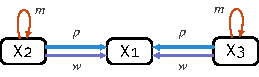
\includegraphics[width=5.5cm,keepaspectratio]{fig_flows1}
\end{center}
\caption{The data flows of program~\ref{lst:simple-dfg-1}.}%
\label{fig:simple-dfg-1}
\end{subfigure}\\[1em]
\begin{subfigure}{.45\textwidth}
\centering\begin{minipage}{.7\textwidth}
\begin{implisting}*[]
X1=1;
while(X2)
  X1=X1+X1
\end{implisting}
\end{minipage}
\caption{An exponential program.}\label{lst:simple-dfg-2}
\end{subfigure}\hfill
\begin{subfigure}{.45\textwidth}
\begin{center}
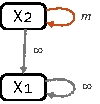
\includegraphics[width=2cm,keepaspectratio]{fig_flows2}
\end{center}
\caption{The data flows of program~\ref{lst:simple-dfg-2}.}%
\label{fig:simple-dfg-2}
\end{subfigure}\\[1em]
\begin{subfigure}{\textwidth}
\centering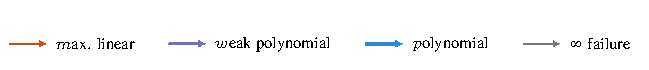
\includegraphics[width=\textwidth,keepaspectratio]{fig_flows3}
\end{subfigure}
\caption[Simple imperative programs and their corresponding data flow graphs]{
Simple \ndx{imperative programs} and their corresponding \ndx{data flow graph}s.
Edges below ∞\symbo{infty} represent acceptable value growth. In the left
program, all variable values grow at most polynomially, \ie satisfactorily. In
the right program, variable \pr|X1| grows exponentially. This is \enquote{too
fast} for a polynomial bound.
}\label{fig:dfg-ex}
\end{figure}

\paragraph*{Analysis result and \ndx{derivability}}
If all final values can be bounded by polynomials, then the input program is
\emph{derivable}. The flow calculus\index{mwp-calculus} assigns an
\emph{\ndx{mwp-bound}} to every variable of a derivable program. An
\ndx{mwp-bound} is an expression, in terms of the inputs, that characterizes the
value growth of a single variable. If a derivable program terminates, the
soundness theorem of the flow calculus~\cite[p. 11]{jones2009}\index{soundness
of mwp-calculus}\index{mwp-calculus} guarantees that the variable value growth
is polynomially-bounded. The result is sound but not complete, \ie not all
satisfactory programs can be captured, but on success we can prove the result
with a derivation. Since the analysis omits \ndx{termination}, this is a
\ndx{partial correctness} guarantee.

The flow calculus\index{mwp-calculus} offers no guarantee to programs that are
not derivable;\index{derivation failure} their variable value growth is
\emph{unknown}. A program always fails if some variable value grows \enquote{too
fast}, \eg exponentially. Failure may also arise from inability to express
satisfactory behavior. This is a built-in limitation of the flow
calculus;\index{mwp-calculus} and more broadly, a common limitation among
related systems~\cite[p. 2]{baillot2015}. The flow calculus alleviates the
issues with nondeterministic\index{nondeterminism} \ndx{inference rule}s. The
\ndx{nondeterminism} increases \ndx{expressiveness}, to capture a larger class
of programs. But one program may admit multiple derivations, which in turn
complicates the analysis procedure. A program is derivable\index{derivability}
if there exists a derivation without an ∞\symbo{infty} coefficient.

\subsubsection{Loop \ndx{specifications} for formal guarantees}
\label{subsec:specs}

Formally verifiable\index{formal verification} programs are defined as precise
mathematical models through \ndx{specifications}. Verifying the program requires
giving a proof that the program satisfies its specification. The motivation for
using \ndx{formal methods} is the strength of guarantees it provides. In
contrast to tests and inspection, a proof conclusively ensures behavioral
correctness at the modeled level of abstraction.

\paragraph*{Specifications}
A {specification}\index{specifications} is a formal contract with three
components.
\begin{enumerate*}

\item \emph{Precondition}\index{precondition} \(P\)\symbo{pre}, is the initial
logic expressions assumed to hold before entering the loop.

\item Program, \pr|loop b C|, performs command \pr|C|\symbo{p2} until the
expression \pr|b| becomes false.

\item \emph{Postcondition}\index{postcondition} \(Q\)\symbo{post}, is the final
logic expressions asserted to hold after the loop terminates.

\end{enumerate*}

Using a \ndx{Hoare triple}~\cite{hoare1969}, we can express the specification as
\(\Hoare{P}{\prm{loop b C}}{Q}\)\symbo{hoare}. The implementation of the program
is correct if we can construct a proof that shows the program satisfies its
specification\index{specifications} in all states. A correctness proof requires
verifying that every computation terminates\index{termination}, every call to
another procedure satisfies its \ndx{precondition}s, and the \ndx{postcondition}
holds at program \ndx{termination}~\cite{furia2010}. For an example of
\ndx{specifications}, refer to Appendix~\ref{app:sec:verified}.

\paragraph*{Relating postconditions and loop \ndx{invariant}s}
A \ndx{postcondition} is a higher-level view describing the program goal. In
case of loops, a \emph{postcondition} is a conditions that must hold after the
loop terminates.\index{termination} The \ndx{postcondition} inference problem
can be expressed informally as follows. Given a \ndx{precondition}
\(P\)\symbo{pre} (in our formulation a constant true, \(\top\))\symbo{ttrue},
and a program \pr|loop b C|, the inference problem involves finding a
postcondition \(Q\)\symbo{post} that satisfies the \ndx{inference rule}
\begin{prooftree} %! suppress = EscapeAmpersand
\hypo{P = \top,
    \Hoare{\prm{b}}{\prm{C}}{\top},
    \lnot\prm{b} \rightarrow Q
    & \vdash \prm{loop b C} }
\end{prooftree}.\symbo{hoare}
Postconditions inferred using the flow calculus\index{mwp-calculus} are provable
by the soundness theorem.\index{soundness of mwp-calculus} However, pre- and
\ndx{postcondition} alone are typically too weak to prove a program correct.
Loop \ndx{invariant}s are needed to make the specification
provable.\index{specifications}

An \emph{\ndx{invariant}} describes an \ndx{assertion} about a program location
that must be true for every program state reaching the
location~\cite{furia2010,nguyen2022}.\footnote{A \ndx{postcondition} is also an
\ndx{invariant}; for clarity, we always refer to a \ndx{postcondition} as such
and use `\ndx{invariant}` to refer to an inductive\index{invariant!inductive}
loop\index{loop invariant} \ndx{invariant}.} A {loop invariant}\index{loop
invariant} is a weakened form of the \ndx{postcondition}~\cite{furia2010}. An
\ndx{invariant} is {inductive} if it holds the first time the location is
reached and is preserved in every cycle returning to the
location~\cite{sankaranarayanan2004}. Verifying loops requires discovering
{sufficiently strong} inductive loop invariants\index{loop invariant} to prove
the specification. For an \ndx{invariant} to be sufficient, it must be weak
enough to be derived from the \ndx{precondition} and strong enough to conclude
the \ndx{postcondition}.

Inductive\index{invariant!inductive} loop\index{loop invariant} \ndx{invariant}s
and \ndx{postcondition}s are symbiotic: the discovery of one assists finding the
other~\cite{furia2010}. Every \ndx{invariant} is necessarily a (weak)
\ndx{postcondition}, as it must hold at \ndx{termination}, but a
\ndx{postcondition} must not be \ndx{invariant}. For example, given natural
numbers \pr|i| and \pr|n|, the loop \prc|for(i=0;i<n;i++) i++;| has an
\ndx{invariant} \(0 \leq \prm{i} \leq \prm{n}\) and a \ndx{postcondition}
\(\prm{i}=\prm{n}\). Invariant inference techniques may assume
\ndx{precondition}s and \ndx{postcondition}s are known. However, this assumption
is impractical, since manually adding \ndx{specifications} to code fragments is
non-trivial.

\subsection{Technical Preliminaries of the Flow Calculus}
\label{sec:calc}

\begin{figure}[H]
\centering
\scalebox{.88}{%! suppress = EscapeHashOutsideCommand
\begin{tikzpicture}[align=center,
arrow/.style={thick,arrows={-Latex[width=6pt, length=4pt]}},
label/.style={midway,fill=white}]
\newcommand\lbl[2]{\textit{#1} (%! suppress = EscapeHashOutsideCommand
\autoref{#2})}
\newcommand\vtx[2]{\textbf{#1} (%! suppress = EscapeHashOutsideCommand
\autoref{#2})}

\path (0, 0) node (A) {\vtx{loop}{subsec:imp-language}}
++(0,-2.0) node[text width=10cm] (B)
    {\vtx{program analysis with flow calculus}{subsec:matrices}}
++(0,-3.7) node (C) {\vtx{evaluation}{sec:enhancements}}
++(0,-3.0) node (D) {\vtx{postconditions}{sec:pc-analysis}};

\draw[cdafny!40!white,line width=5pt,solid]
    ($(C.north west)+(-1.5,0.4)$)  rectangle
    ($(D.south east)+(1.5,-0.4)$);
\draw[black,thick,densely dashed,line cap=round]
    ($(C.north west)+(-1.5,0.4)$)  rectangle
    ($(D.south east)+(1.5,-0.4)$);

\draw [arrow,sbase03,arrows={
    {Circle[open]}-Latex[width=6pt, length=4pt]}] (A) -- (B) ;
\draw [arrow,sbase03] (B) -- node[label,yshift=7pt]
    {\lbl{mwp-matrix}{subsec:mat-decode}} (C);
\draw [arrow,sbase03] (C) -- node[label]
    {\lbl{mwp-bounds}{subsec:interpreting-mwp-bounds}}(D);
\end{tikzpicture}}

\caption[The mwp-analysis workflow]
    {The mwp-analysis workflow.\index{mwp-calculus}}
\label{fig:pc-workflow}
\end{figure}

The \autoref{fig:pc-workflow} illustrates the complete analysis workflow.
The boxed region highlights the steps and enhancements introduced in this paper.
The region outside the box refers to the existing techniques we build on.

The analysis takes as input an imperative loop \index{imperative programs}
(\autoref{subsec:imp-language}). We analyze the loop using the \ndx{inference
rule}s of the flow calculus (\autoref{subsec:matrices})\index{mwp-calculus}. As
output, the analysis produces an \emph{\ndx{mwp-matrix}}
(\autoref{subsec:mat-decode}). Our enhancements involve {evaluating} these
mwp-matrices. We define first an {evaluation procedure} (\autoref{subsec:eval})
that enables extracting optimal \ndx{mwp-bound}s from mwp-matrices, and in more
cases than previously (\autoref{subsec:bounds-at-failure}). This provides the
\ndx{postcondition}s that address the problem formulation
of~\autoref{subsec:overview}.

\subsubsection{Imperative language of input programs}
\label{subsec:imp-language}

\begin{definition}[Imperative language]
\label{def:lang}\index{imperative programs}
Letting natural number variables range over \pr|X| and \pr|Y| and Boolean
expressions over \pr{b}, we define \emph{expressions} \pr|e|, and
\emph{commands} \pr|C| as follows
%! suppress = MissingImport
\begin{align*}
    \text{\pr|e|} \coloneqq{ }&
    \text{\pr| X|} \BNF
    \text{\pr|X - Y|} \BNF
    \text{\pr|X + Y|} \BNF
    \text{\pr|X * Y|} \\
    \text{\pr|C|} \coloneqq{ }&
    \text{\pr| skip|} \BNF
    \text{\pr|X = e|} \BNF
    \text{\pr|if b then C else C|} \BNF
    \text{\pr|while b C|} \BNF
    \text{\pr|loop X C|} \BNF
    \text{\pr|C;C|}
\end{align*}\symbo{coloneqq}\symbo{bnfsep2}
The command \pr|loop X C| means \enquote{do \pr|{C}| \pr|X| times} and the
variable \pr|X| is not allowed to occur in command \pr|C|. Command \pr|C;C| is
for sequencing. We write \enquote{program} for a series of commands composed
sequentially. \end{definition} We implicitly convert between conventional
\prc|for| loops and \pr|loops| of the imperative language in examples. The
values of Boolean expressions do not matter. For emphasis, we substitute \pr|b|
with \pr|*| in control expressions. Although the base language is rudimentary,
it captures a core fragment of conventional mainstream programming languages,
like \ndx{C} and \ndx{Java}. Our technique applies to all languages sharing the
same core, including intermediate representations\index{intermediate
representation}. Similarly, the approach is applicable even if a programming
language provides little structure.

\subsubsection{About construction of mwp-matrices}
\label{subsec:matrices}

How mwp-matrices\index{mwp-matrix} are constructed is not crucial for the
developments of this paper. The construction procedure is well-established in
literature~\cite[Sect. 5--6]{jones2009} and~\cite[Sect.
2--3]{aubert20222}.\footnote{Our work assumes the variant described
in~\cite{aubert20222}.} We give a brief overview, but make no adjustment to the
construction procedure. Rather, mwp-matrices\index{mwp-matrix} are our inputs of
interest. We focus on \emph{interpreting} the information they encode.

During matrix construction, the flow calculus\index{mwp-calculus} assigns
matrices to commands of the input program. The procedure resembled typing,
except the \enquote{types} are complicated matrices.\index{matrix-as-type} An
\emph{mwp-matrix} \(M\)\symbo{matrix} captures data flow facts about the
analyzed program \(\mathcal{C}\)\symbo{prog2}. The matrices track, through flow
coefficients,\index{flow coefficient} how data flows in variables between
commands. What coefficients are assigned is determined by the \emph{inference
rules} of the flow calculus. The relevant inference rules are included in
Figures~\ref{fig:rules-expressions} and~\ref{fig:rules-loops}.\footnote{ To ease
the presentation, we show rules of the original flow calculus~\cite{jones2009}.
These rules are consistent with the enhanced variant~\cite{aubert20222} we build
on.} To trade \ndx{precision} for efficiency, the flow
calculus\index{mwp-calculus} omits evaluating loop iteration bounds and
reasoning about \ndx{termination} and control expressions, overestimating their
effect. At conclusion, the flow calculus assigns \underline{one}
\ndx{mwp-matrix} to the analyzed program, \(\vdash\mathcal{C} : M\)\symbo{cmat}.
It contains all derivations of the input program in one (complex) data
structure.

\begin{figure}[h]
\begin{tabularx}{\textwidth}{CCC}
%! suppress = EscapeUnderscore
\begin{prooftree}[small, center=false]
\infer0[E2]{
\vdash \prm{e} : \{_{\,i}^{w} \mid \prm{X}_i \in \var(\prm{e}) \}}
\end{prooftree}\symbo{xvar}\symbo{vare}\symbo{v0a}\symbo{evec}
&
%! suppress = EscapeUnderscore
\begin{prooftree}[small, center=false]
\hypo{\vdash \prm{X}_i : V_1}
\hypo{\vdash \prm{X}_j : V_2}
\infer2[E3]{\vdash \prm{X}_i + \prm{X}_j : pV_1 \oplus V_2}
\end{prooftree}\symbo{xvar}\symbo{p}\symbo{vec}\symbo{evec}
&
%! suppress = EscapeUnderscore
\begin{prooftree}[small, center=false]
\hypo{\vdash \prm{X}_i : V_1}
\hypo{\vdash \prm{X}_j : V_2}
\infer2[E4]{\vdash \prm{X}_i + \prm{X}_j : V_1 \oplus pV_2}
\end{prooftree}\symbo{xvar}\symbo{p}\symbo{vec}\symbo{evec}
\symbo{xi}\symbo{oplus}
\end{tabularx}
\caption[A selection of flow calculus rules for assigning vectors to
expressions.]{
A selection of flow calculus\index{mwp-calculus} rules for assigning vectors to
expressions. A {variable} is denoted as \(\prm{X}_i\)\symbo{xvar} where the
\(i\) refers to an index of a matrix column (\resp \(\prm{X}_j\) for the \(j\)th
column). In rules E3 and E4, a vector of coefficients is denoted by
\(V_n\)\symbo{vec}. In other words, the rules assign vectors of coefficients to
variables. Three rules can be used to analyze a single expression. The
\ndx{nondeterminism} of the flow calculus\index{mwp-calculus} comes from these
\ndx{inference rule}s.}
\label{fig:rules-expressions}
\end{figure}

Nondeterminism\index{nondeterminism} is necessary to improve the expressive
power\index{expressiveness} of the flow calculus\index{mwp-calculus}, but
complicates the analysis procedure. There are the three rules
(\autoref{fig:rules-expressions}) to analyze an expression of binary
addition\footnote{ Similar rules exist for subtraction, and multiplication is
always handled by E2.}, like \pr|X1 + X2|. Informally, the rule E2 says
\enquote{we can always assign a \(w\)\symbo{w} coefficient to all variables in
the expression}. Although such constant treatment seems  potentially harmful,
the \ndx{inference rule}s for analyzing commands (\autoref{fig:rules-loops})
ensure only acceptable data flow patterns are accepted as
derivable.\index{derivability} The rule E3 says \enquote{the vector of the left
operand is multiplied by a polynomial coefficient.} The
\(p\)\symbo{p}-coefficient tracks the fact that certain data flow patterns might
not be polynomially bounded~\cite[p. 13]{jones2009}. Applying the rules to a
vector propagates the effect to all variables that are transitively dependent on
the left operand. Rule E4 is similar to E3, except the \(p\)\symbo{p}
coefficient is applied to the right operand. Thus, three different derivation
can arise from one expression, and from every command that contains the
expression. Going forward, we omit the details of these rules and instead refer
to them by a mapping \(0 \mapsto \text{E4}, 1 \mapsto \text{E3}, 2 \mapsto
\text{E2}\)\symbo{map}.

\subsubsection{Our starting point of interest: interpreting mwp-matrices}
\label{subsec:mat-decode}

An \ndx{mwp-matrix} represents the derivations of an analyzed program. Before
diving into full mwp-matrices\index{mwp-matrix}, this section describes its
\emph{elements}.

\paragraph*{Basic terms}
Flow coefficients---described in \autoref{subsec:flow-calc-intro}---are the core
building blocks of mwp-matrices. The \ndx{flow coefficient}s are elements of the
finite set \(\text{\textsc{mwp}}^\infty \triangleq \{0, m, w,
p,\infty\}\)\symbo{mwpi}\symbo{zero}\symbo{m}\symbo{w}\symbo{p}\symbo{infty}. A
\emph{domain} \(\mathcal{D} \triangleq \{0, 1, 2 \}\)\symbo{domain}\symbo{trieq}
is a bidirectional map of the flow calculus\index{mwp-calculus} \ndx{inference
rule}s. In other words, the domain members can be translated to flow calculus
\ndx{inference rule}s (E2--E4) and vice versa. The \emph{degree} of choice, \(k
: \mathbb{N}\)\symbo{k2}\symbo{nat}, is a counter of derivations. The degree
represents the number of times a \ndx{derivation choice} must be made during
program analysis. The degree is precisely equal to the count of binary
arithmetic operations (where the operator is either \(+\) or \(-\)).

\begin{definition}[Derivation choice]
Letting \( \mathcal{D} \)\symbo{domain} be a domain and \( k \in \mathbb{N}
\)\symbo{nat}\symbo{k2} be the degree of choice, we define a \ndx{derivation
choice} as \( \delta(i, j) \)\symbo{delta}, where \( i \subseteq \mathcal{D} \)
and \( j \leq k \).
\end{definition}
A \ndx{derivation choice}, denoted by \(\delta\)\symbo{delta}, represents the
\ndx{nondeterminism} of the flow calculus\index{mwp-calculus}. We call
\(i\)\symbo{mi} the \emph{value} and \(j\)\symbo{mj} the \emph{index} of the
derivation choice. Informally, it captures that an inference rule \(i\) is
applied at program point \(j\).

\begin{definition}[Derivation choice sequence]
Letting \(k\)\symbo{k2} be the degree of choice, we define a \ndx{derivation
choice} sequence as \(\Delta = (\delta_1, \delta_2, \dots,
\delta_{k'})\)\symbo{Delta} where \(0 \leq k' \leq k \).
\end{definition}

Since a program is a \emph{series} of commands, correspondingly we must have
\emph{sequences} of \ndx{derivation choice}s, denoted as
\(\Delta\)\symbo{Delta}. Simple data flow patterns do not require making
\ndx{derivation choice}s; therefore \(\Delta\)\symbo{Delta} can be empty. There
are two restrictions on \(\Delta\)\symbo{Delta}. First, an index \(j\)\symbo{mj}
is allowed to occur at most once in a sequence, \ie the indices in a sequence
must be unique. Second, the sequence is sorted by the index in ascending order.
These restrictions support efficient computation during matrix\index{mwp-matrix}
construction. Since we are only concerned with {interpreting}
mwp-matrices\index{mwp-matrix}, we assume every \(\Delta\)\symbo{Delta}
satisfies the uniqueness and order properties by construction. By
\autoref{fig:rules-expressions}, it is evident that one variable can be assigned
multiple \ndx{flow coefficient}s. The fact that \(\Delta\)\symbo{Delta} reduces
to a particular coefficient is represented in a \emph{\ndx{monomial}}.

\begin{definition}[Monomial]\label{def:mono}
Letting \(\alpha \in \text{\textsc{mwp}}^\infty\)\symbo{alpha}\symbo{mwpi} be a
coefficient and \(\Delta\)\symbo{Delta} be a sequence of \ndx{derivation
choice}s, we define a \ndx{monomial} as \((\alpha,
\Delta)\)\symbo{alpha}\symbo{Delta}.
\end{definition}

\noindent
A \ndx{monomial} in the flow calculus is disjoint from the classic notion of
\ndx{monomial}s. For example, both \(m.(\delta(0,0),\delta(2,1))\)\symbo{delta}
and \(0\)\symbo{zero} are valid \ndx{monomial}s by definition. The former says
\enquote{if we apply rule 0 then rule 2 (at indices 0 and 1, resp.) then we
obtain an \(m\)\symbo{m} coefficient}. The latter says \enquote{no matter the
choice, we always obtain a \(0\)\symbo{zero} coefficient}. Finally, the fact
that different \(\Delta\)\symbo{Delta} reduce to different
coefficients\index{flow coefficient} is represented by a \emph{\ndx{polynomial
structure}}.

\begin{definition}[Polynomial structure]
We define a \ndx{polynomial structure} as a sequence of \ndx{monomials}
\(\big(0,(\alpha_1,\Delta_1)\), \((\alpha_2,\Delta_2)\), \(\dots\), \((\alpha_m,
\Delta_m)\big)\) where \(m \geq 0\).\symbo{alpha}\symbo{Delta}
\end{definition}

\noindent The \ndx{polynomial structure} is prefixed by
\(0\)\symbo{zero}-\ndx{monomial} to ensure it is always non-empty. \textbf{The
elements of an mwp-matrix are \ndx{polynomial structure}s.}

\subsubsection{Decoding an mwp-matrix by example}
\label{subsec:read-mat}

An \ndx{mwp-matrix} \(M\)\symbo{matrix} associates variables with
\ndx{polynomial structure}s.\footnote{ For clarity and compactness, we omit
needless \(0\)\symbo{zero}'s, \(\delta\)\symbo{delta}-symbols, and delimiters
when displaying mwp-matrices.} This association is defined by position. The
matrix size is determined by the number of program variables, such that for
\(n\) variables, the matrix size is \(n \times n\). The matrix is labelled by
the variables. An mwp-matrix is interpreted {column-wise}. The data-flow facts
about a variable at column \(j\)\symbo{mj} are collected in the \ndx{polynomial
structure}s at rows \(i=(1, \ldots, n)\) in \(M_{ij}\).

\begin{example}[mwp-matrix of \explain]\label{ex:mat}
Consider the \ndx{mwp-matrix} of \explain.

\begin{center}
\begin{minipage}{\linewidth}
\begin{minipage}{.28\linewidth}
\begin{implisting}*[label={lst:pt-fail},escapeinside=||]
for(i=0;i<X1;i++)
{ X3=X2*X2;
  X3=X3+X5; |\circledc{1}|
  X4=X4+X5; |\circledc{2}| }
\end{implisting}
\end{minipage}%
\hfill : \hfill%
\scalebox{.8}{\(%! suppress = EscapeAmpersand
\begin{pNiceMatrix}[first-row,first-col]
& \prm{X1} & \prm{X2} & \prm{X3} & \prm{X4} & \prm{X5} \\
\prm{X1} & m & 0 & p(0,0),p(1,0)         & p(0,1),\infty(1,1),\infty(2,1)  & 0 \\
\prm{X2} & 0 & m & w(0,0),p(1,0),w(2,0)  & \infty(1,1),\infty(2,1)         & 0 \\
\prm{X3} & 0 & 0 & m                     & \infty(1,1),\infty(2,1)         & 0 \\
\prm{X4} & 0 & 0 & 0                     & m,\infty(1,1),\infty(2,1)       & 0 \\
\prm{X5} & 0 & 0 & p(0,0),m(1,0),w(2,0)  & p(0,1),\infty(1,1),\infty(2,1)  & m \\
\end{pNiceMatrix}\)}\symbo{xvar}\symbo{zero}\symbo{m}\symbo{w}\symbo{p}\symbo{infty}
\end{minipage}
\end{center}

We mark the program points where a \ndx{derivation choice} must be made as
\circledc{1} and \circledc{2}. The program points correspond to indices 0 and 1,
respectively. These points give the \ndx{mwp-matrix} a degree of 2. The addition
expressions are analyzed by the \ndx{inference rule}s
of~\autoref{fig:rules-expressions}. The mwp-matrix contains derivations choices
at columns \pr|X3| and \pr|X4| because they are the data-flow targets of the
additions. Correspondingly, in~\autoref{fig:ll-dfg}, the variables are targets
of dependence edges.

\begin{figure}[H]
\centering
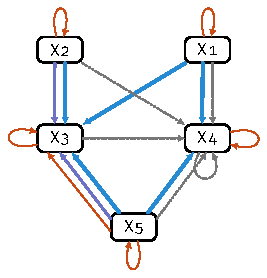
\includegraphics[width=6cm,keepaspectratio]{fig_lucid}
\caption[A data-flow graph of \exname]{A data-flow graph of \exname.}
\label{fig:ll-dfg}
\end{figure}

\noindent{}Variables \pr|X1|, \pr|X2|, and \pr|X5| are assigned at most
\(m\)\symbo{m}{ }coefficients\index{flow coefficient}. An \(m\)-flow at the \ndx{mwp-matrix} diagonal
means the variable depends on its (own) initial value. Since the program has no
commands that would introduce multiple derivations on these variables, their
\ndx{polynomial structure}s are simple coefficients. Variable \pr|X3| shows
varying dependencies on \pr|X1|, \pr|X2|, and \pr|X5| at corresponding rows. The
coefficients\index{flow coefficient} indicate that the dependencies are at most
polynomial (similarly observable in the \textsc{dfg}). The absence of
∞\symbo{infty} means the value growth of \pr|X3| is acceptable in all
derivations. Variable \pr|X4| is assigned ∞\symbo{infty} in some derivations.
Intuitively, this is because the value of \pr|X4| accumulates at each loop
iteration and its value growth is potentially problematic. The
∞-flow\symbo{infty} signals that some derivations fail\index{derivation failure}
and flags \pr|X4| as the source of failure. However, this is the current extent
of our capabilities to describe \pr|X4|~\cite{aubert2023b}.
\end{example}

\noindent This paper develops enhanced strategies to extract more precise
information from mwp-matrices.\index{mwp-matrix} $\poly_2$\symbo{hp}Although we
show only compact cases, an mwp-matrix captures \(3^k\) \ndx{derivation choice}s where
\(k\)\symbo{k2} is the degree. Clever solutions are necessary to explore and
interpret the \ndx{mwp-matrix} data efficiently, but have been missed by
previous flow calculus\index{mwp-calculus}
refinements~\cite{aubert20222,aubert2023b}.

\subsubsection{Interpreting mwp-bounds}
\label{subsec:interpreting-mwp-bounds}

The \ndx{mwp-matrix} columns encode the variable value growth bounds. An
mwp-bound is an expression of form $\max(\vec{x}, \poly_1(\vec{y})) +
\poly_2(\vec{z})$\symbo{hp}\symbo{vlist}. Variables characterized by
$m$\symbo{m}-flow are listed in $\vec{x}$; $w$\symbo{w}-flows in $\vec{y}$, and
$p$\symbo{p}-flows in $\vec{z}$. Variables characterized by $0$\symbo{zero}-flow
do not occur in the expression. No bound exists if some variable is
characterized by ∞\symbo{infty}\index{derivation failure}. The
$\poly_1$\symbo{hp} and  are \emph{\ndx{honest polynomial}s}, build up from
constants and variables by applying $+$ and $\times$. The variables with
\(w\)\symbo{w}-flow occur in $\poly_1$\symbo{hp} and variables with
\(p\)\symbo{p}-flow in $\poly_2$\symbo{hp}. Any of the three variable lists
might be empty, and $\poly_1$ and $\poly_2$\symbo{hp} may not be present. When
characterizing value growth, an \ndx{mwp-bound} is approximative. It excludes
precise constants and degrees of polynomials. An \ndx{mwp-bound} is a monotonic
over-approximation, \ie it does not decrease if variable value decrease over
subtraction. A program \emph{bound} is a conjunction of its variables'
\ndx{mwp-bound}s. \autoref{ex-bounds} shows illustrative cases of
\ndx{mwp-bound}s. The differences between the bound forms are discussed in
Sections~\ref{subsec:categories} and~\ref{subsec:disclaimer}.

\begin{note}
For variable \pr|X|\symbo{xvar} and an \ndx{mwp-bound} \(W\)\symbo{bound},
we write \(\prm{X'} \leq W\)\symbo{Xprime} to denote the \ndx{mwp-bound} of
variable \pr|X|. We use the overloaded notation \pr|X'| to refer to the
variable's final value. Variables in \(W\)\symbo{bound} always refer to
initial values.
\end{note}

\begin{example}\label{ex-bounds}
The \ndx{mwp-bound} (on left) is interpreted as, {the \emph{final value}
of\ldots}

\noindent\hfill\begin{tabular}{@{}rl@{\hskip 0.1in}l@{}}
\(\prm{X2'} \leq \prm{X2} \) & & {\ldots \prc|X2| is bounded linearly by its
initial value.} \\
\(\prm{X3'} \leq \max(\prm{X3},\prm{X2}+\prm{X5})\) & & {\ldots \prc|X3| is
bounded by a weak polynomial in \prc|X3| or \(\prm{X2}+\prm{X5}\).} \\
\(\prm{X4'} \leq \max(\prm{X4})+\prm{X1}\times\prm{X5}\) & & {\ldots \prc|X4| is
bounded by a polynomial in \prc|X4| and \(\prm{X1}\times\prm{X5}\).}
\end{tabular}
\end{example}

\subsection{Variable-Guided Matrix Exploration}
\label{sec:enhancements}

\subsubsection{Addressed limitations}
\label{subsec:enhancements}

We introduce two solutions to address current limitations of the flow
calculus.\index{mwp-calculus}

\begin{enumerate}

\item An \ndx{mwp-matrix} \emph{evaluation strategy}, to efficiently determine
if an individual variable admits an \ndx{mwp-bound} of specific form.

\item Improved \emph{derivation failure handling}, to identify variables that
maintain acceptable value growth in presence of whole-program \ndx{derivation
failure}.

\end{enumerate}

\noindent The \ndx{nondeterminism} of the flow calculus\index{mwp-calculus}
permits capturing more programs, but creates a potential \ndx{state explosion}
problem. Effectively handling this aspect becomes critical in the second
analysis phase, where an mwp-matrix is \emph{evaluated} to find \ndx{mwp-bound}s
of variables. The first challenge is finding the \ndx{derivation choice}s that
do not produce failure. The second challenge is determining the
coefficients\index{flow coefficient} assigned to each variable. The coefficients
are not obvious from the \ndx{derivation choice}s of an \ndx{mwp-matrix};
rather, they require an application. An \emph{application} reduces the
\ndx{polynomial structure}s to simple coefficients\index{flow coefficient},
which then leads to \ndx{derivation failure} or yields a program bound.

A brute force solution iterates all derivations and applies all choices to
observe the result. However, such naive solution is impractical, due to latency
and a potential yield of exponentially many program bounds. The ideal solution
should find the optimal bound (if one exists) and without the redundancy of
iterating every derivation.

The evaluation strategy we present operates as follows. It takes the
\emph{unwanted} \ndx{derivation choice}s then negates them. The evaluation
result the captures the \emph{permissible} choices. The term permissible is
abstract -- the meaning depends on what is unwanted. For example, if the
\ndx{derivation choice}s of ∞ coefficients\index{flow coefficient} are unwanted,
the permissible choices are those that avoid failure, \ie non-∞. The result of
an evaluation is a \emph{disjunction of \ndx{choice vector}s} that compactly
capture the permissible \ndx{derivation choice}s.

\begin{definition}[Choice vector]
Letting \( \mathcal{D} \)\symbo{domain} be a domain and \( k \in \mathbb{N}
\)\symbo{nat}\symbo{k2} be a choice degree, we define a choice vector as \(
\vec{C} = (c_1, c_2, \ldots, c_k) \)\symbo{cv}, where \( c_i \subseteq
\mathcal{D} \) and \( c_i \neq \emptyset \) for all \( i \in \{1, 2, \ldots, k\}
\).
\end{definition}
We show \ndx{choice vector}s in Examples~\ref{ex:derivable},~\ref{ex:wbound},
and~\ref{ex:whl}.

\subsubsection{Evaluation for identifying derivable programs}
\label{subsec:eval}

The precise mwp-matrix evaluation strategy is presented in~\autoref{alg:algo}
and we describe it here informally. The evaluation is parametric on three
inputs:
\begin{enumerate*}[label=(\roman*)]
\item the degree of choice \(k\)\symbo{k2},
\item domain \(\mathcal{D}\)\symbo{domain}, and
\item a set of unwanted \ndx{derivation choice}-sequences, \(\mathcal{S} =
\{\Delta_1,\ldots,\Delta_n\}\)\symbo{dset} where \(n \geq 0\).
\end{enumerate*}
Observe that all parameters are obtained from an \ndx{mwp-matrix}, but the
mwp-matrix or its coefficients\index{flow coefficient} are \underline{not} used.
The evaluation returns a list of \ndx{choice vector}s. In the maximally
permissive case, the result is a single \ndx{choice vector} permitting
everything. If no result exists or no choice is necessary, the result is an
empty list. These outcomes are handled as base cases
(Lines~\ref{alg:step0}--\ref{alg:step0end}). All interesting evaluations fall
between these extremes.

\begin{algorithm}
    \caption{\ndx{mwp-matrix} evaluation}
    \label{alg:algo}
    \textbf{Input}:
    degree \(k\) (\(\mathbb{N}\))\symbo{k2}\symbo{nat},
    domain \(\mathcal{D}\)\symbo{domain} (set),
    derivation choice-sequences \(\mathcal{S}\)\symbo{dset} (set)\\
    \textbf{Output}: \ndx{choice vector}s \(\mathcal{C}\)\symbo{cvl} (list)
    \begin{algorithmic}[1]
        \State \(\mathcal{C} \gets \varepsilon \)
        \LineComment{Handle base cases}
        \If {\(k = 0\) \textbf{or} \(|\mathcal{D}|\leq 1\) \textbf{or} \(\mathcal{S} = \emptyset\)}\label{alg:step0}
        \If {\(\mathcal{S} = \emptyset\)}
            \State Create \(\vec{c} \coloneqq\)\symbo{coloneqq} ChoiceVector(\(k, \mathcal{D}\))
            \Comment{\(k\)-length vector of elements in \(\mathcal{D}\)}
            \State \(\mathcal{C} \gets \vec{c} \dblcolon\mathcal{C} \)
        \EndIf
        \State \Return \(\mathcal{C}\)\label{alg:step0end}
        \EndIf
        \LineComment{Step 1: Simplify \(\mathcal{S}\) until convergences}
        \Do \; Capture initial \(\text{\textit{size}} \coloneqq |\mathcal{S}|\)
        \Comment{\(\mathcal{O}(\mathcal{S}^3)\)}
        \State \(\mathcal{S} \gets \textsc{Simplify}(\mathcal{S})\)\label{alg:step1}
        \doWhile{\text{\textit{size}} \(\neq |\mathcal{S}|\)}
        \LineComment{Step 2: Generate \ndx{choice vector}s}
        \State Compute \(P \coloneqq\) the product of sequences in \(\mathcal{S}\)\label{alg:step2}
        \ForAll{paths \(p\) in P} \Comment{\(\mathcal{O}\left(\prod_{s \in \mathcal{S}} |s|\right)\)}
        \State Create \(\vec{c} \coloneqq\)\symbo{cv} ChoiceVector(\(k, \mathcal{D}\))
        \ForAll{\((i, j)\) in \(p\)}  \Comment{\(\mathcal{O}(|\mathcal{S}|)\)}
        \State Remove \(i\) at \(\vec{c}_j\)
        \EndFor
        \If {\(\forall j, \vec{c}_j \neq \emptyset \)}
            \State \(\mathcal{C} \gets \vec{c} \dblcolon\mathcal{C} \)\label{alg:add}\label{alg:step2end}
        \EndIf
        \EndFor
        \State \Return \(\mathcal{C}\)
    \end{algorithmic}
\end{algorithm}

The evaluation operates in two steps. First it simplifies
\(\mathcal{S}\)\symbo{dset} to the minimal length, non-empty sequences while
preserving its effect. Then, it generates the \ndx{choice vector}s by negating
the remaining unwanted choices. The procedure is practically efficient because
simplification eliminates redundancy before the \ndx{choice vector} are
generated. Internally, it benefits from the finiteness of the domain and from
having advance complete knowledge of all \ndx{derivation choice}s.

The simplification step (Line~\ref{alg:step1}) is crucial. It must be
sound\index{soundness} and complete\index{completeness} to ensure all distinct
derivation patterns are preserved in \(\mathcal{S}\)\symbo{dset}, but also
reduces \(\mathcal{S}\)\symbo{dset} to a minimal set. Different simplifications
are applied on \(\mathcal{S}\)\symbo{dset} iteratively until convergence,
including the following.

\begin{description}

\item[Remove super-sequences.] When a sequence leads to an unwanted outcome,
every longer sequence producing the same outcome is redundant. For example, if
\(\mathcal{S}\)\symbo{dset} contains \(((0,0),(0,1),(1,2))\) and \(((0,1))\) we
remove the longer sequence.

\item[Head-elimination.] If many non-singleton sequences differ only on their
head element value, and the values cover the domain \(\mathcal{D}\), then the
head is redundant. The sequences can be replaced by one sequence without the
head element. For example, the sequences \(((0,0)(1,1))\), \(((1,0)(1,1))\),
\(((2,0)(1,1))\) can be replaced by \(((1,1))\).

\item[Tail-elimination.] By symmetry, the same as above, but on the tail
element.

\end{description}

The generation step (Lines~\ref{alg:step2}--\ref{alg:step2end}) produces the
\ndx{choice vector}s. They are constructed by computing the cross product of
\(\mathcal{S}\)\symbo{dset}. We take one \ndx{derivation choice} from each
sequence, then eliminating those choices. This prevents choosing any unwanted
sequence completely. If the \ndx{choice vector} elements are non-empty after
elimination, we appended the \ndx{choice vector} to the result
(Line~\ref{alg:add}). We have annotated the computational costs of the iterative
steps in~\autoref{alg:algo}. The algorithm obviously
terminates.\index{termination} Since the generation step involves a product, it
is a source of potential inefficiency. However, we have not encountered natural
programs where the simplification does not reduce \(\mathcal{S}\)\symbo{dset}
sufficiently to make the generation step problematic. A full implementation of
the algorithm is included in our artifact, and described in the
\href{https://statycc.github.io/pymwp/choice}{documentation} of
\ndx{pymwp}.\footnote{See: \url{https://statycc.github.io/pymwp/choice}}

\begin{example}[\exname is derivable]\label{ex:derivable}
In \autoref{ex:mat}, the distinct \ndx{monomial}s that cause failure are
\(\infty.\delta(1,1)\)\symbo{delta}\symbo{infty} and  \(\infty.\delta(2,1)\).
The mwp-matrix degree is \(k=2\)\symbo{k2}, the domain is
\(\mathcal{D}=\{0,1,2\}\)\symbo{domain}, and the unwanted \ndx{derivation
choice}-sequences are \(\mathcal{S} = \{ ((1,1)), ((2,1)) \}\)\symbo{dset}. The
evaluation returns a choice vector \(\big(\{0,1,2\}, \{0\}\big)\) witnessing
successful \ndx{derivation choice}s. The choice vector communicates that we can
select any derivation rule to analyze command \circledc{1}, but must apply
\enquote{inference rule 0} (E4) at command \circledc{2}.
\end{example}

The application of a \ndx{choice vector} requires making a selection at each
vector index, then applying the selections to the \ndx{polynomial structure}s of
the \ndx{mwp-matrix}. A \ndx{monomial} evaluates to \(\delta(i, j) =
\alpha\)\symbo{delta}\symbo{alpha} if the \(j\)\symbo{mj}th choice is
\(i\)\symbo{mi}, and \(0\)\symbo{zero} otherwise. A polynomial structure
evaluates to its maximal coefficient\index{flow coefficient}. Thus, the
application produces the maximal coefficient among the \ndx{monomial}s
(\cf~\autoref{ex:whl}).

\subsubsection{Variable projection and querying mwp-bounds}
\label{subsec:query}

Until now, the flow calculus\index{mwp-calculus} of mwp-bounds has been
restricted to deriving \ndx{mwp-bound}s for all variables concurrently. For
\ndx{postcondition} inference, we want to obtain information about
\emph{individual} variables. Since~\autoref{alg:algo} does not require
mwp-matrices\index{mwp-matrix} or coefficients\index{flow coefficient} as
input, it can be directly reused for variable-specific evaluations.

Analyzing variable \(\prm{X}_j\)\symbo{xvar} requires taking \ndx{derivation
choice}s only from column \(j\)\symbo{mj}, instead of the entire
\ndx{mwp-matrix}. To determine if a variable admits a particular form of
\ndx{mwp-bound}, we issue \enquote{queries} against the evaluation procedure,
altering the \ndx{derivation choice}s provided as parameter
\(\mathcal{S}\)\symbo{dset}. For example, to find derivations with at most
\(m\)\symbo{m} coefficients (and whether they exist), we take the
\ndx{derivation choice}s from \ndx{monomial}s whose coefficient are in \(\{w,
p,\infty\}\).\symbo{w}\symbo{p}\symbo{infty} If the evaluation returns a
\ndx{choice vector}, it specifies the derivations where the variable is assigned
an mwp-bound of at most \(m\)\symbo{m} coefficients.\index{flow coefficient}
Bounds with at most \(w\) or \(p\)\symbo{w}\symbo{p} can be queried similarly,
by adjusting \(\mathcal{S}\)\symbo{dset}.

\begin{example}
[Variable \texttt{X3} is bounded by at most $w$ coefficients]
\label{ex:wbound}
In \autoref{ex:mat}, variable \pr|X3| does not have a derivation with at most
\(m\)\symbo{m} coefficients. This can be determined by evaluation of the
distinct choices in column \pr|X3| with \(\{w, p,
\infty\}\)\symbo{p}\symbo{infty} coefficients\index{flow coefficient}, \ie
\(\mathcal{S} = \{ ((0,0)),((1,0)),((2,0)) \}\)\symbo{dset}. This evaluation
does not return a \ndx{choice vector}. However, an \ndx{mwp-bound} of at most
\(w\)\symbo{w} exists, by the \ndx{choice vector} \(\big(\{2\},
\{0,1,2\}\big)\).
\end{example}

\noindent Variable query is safe for derivable programs\index{derivability},
because all variables are guaranteed to have an \ndx{mwp-bound} by the soundness
theorem of the flow calculus~\cite[p. 11]{jones2009}.\index{soundness of
mwp-calculus} Additional caution is needed when a program is not derivable.

\subsubsection{Variable mwp-bounds in presence of failure}
\label{subsec:bounds-at-failure}

Derivation failure\index{derivation failure} arises from the \ndx{inference
rule}s of commands \pr|while| and \pr|loop|, in~\autoref{fig:rules-loops}.

%! suppress = EscapeUnderscore
\begin{figure}[h]
\begin{center}
\begin{prooftree}[small]
\hypo{\vdash \text{\pr|C|} : M}
\infer[left label={\(\forall i, M_{ii}^* = m\)}]1[L]{
\vdash \prm{loop X}_\ell\,\prm{\{C\}} :
M^* \oplus \{_\ell^{p}\rightarrow j \mid \exists i, M_{ij}^* = p\}}
\end{prooftree}
\\[1.2em]
\begin{prooftree}[small]
\hypo{\vdash \text{\pr|C|} : M}
\infer[left label={\(\forall i, M_{ii}^* = m\) and
\(\forall i, j, M^*_{ij} \neq p\)}]1[W]
{\vdash \text{\pr|while b do  \{C\}|} : M^*}
\end{prooftree}
\end{center}
\symbo{matrix}\symbo{cmat}\symbo{xvar}\symbo{closure}\symbo{xi}
\symbo{xj}\symbo{p}\symbo{m}\symbo{mi}\symbo{mj}\symbo{mzeroj}
\symbo{mstar}\symbo{oplus}
\caption[Flow calculus inference rules for \pr|while| and \pr|loop|]{
The flow calculus\index{mwp-calculus} \ndx{inference rule}s for commands
\pr|while| and \pr|loop|.}
\label{fig:rules-loops}
\end{figure}

The interesting parts about these rules are the side conditions. For the
\pr|loop| rule (L), the side condition says a loop can be analyzed if the
flow coefficients\index{flow coefficient} at the \ndx{mwp-matrix} diagonal are at most
\(m\)\symbo{m}. The \pr|while| (W) rule is more restrictive. In addition to
diagonal \(m\)\symbo{m}, no \(p\)\symbo{p} coefficients are allowed to occur
anywhere in the \ndx{mwp-matrix}. These side conditions ensure variable values
grow at most polynomially over repeated executions of the command body.

A program that does not satisfy the side conditions is not
derivable.\index{derivability} Then, variable value growth is inconclusive and
no bound is assigned to its variables. The flow calculus\index{mwp-calculus}
offers no guarantees to programs that are not derivable. A single rogue variable
can cause a whole-program \ndx{derivation failure}. This treatment of failure
limits the utility of the analysis. Since our goal is to infer
\ndx{postcondition}s of loops, this restriction excludes many programs we want
to analyze.

\paragraph*{Improving the failure handling}
Our intuition is that the mwp-matrices\index{mwp-matrix} accumulate information
that permits reasoning about {certain variables} in presence of
failure.\index{derivation failure} The main new idea is to \emph{isolate the
failing variables} from those with acceptable behavior. If such isolation is
possible, then the remaining variables can be analyzed. The idea is conservative
because it does not change the rules of the flow calculus.\index{mwp-calculus}
Rather, the improvement is based on leveraging fully the information already
collected in mwp-matrices.\index{mwp-matrix} We make only the analytical
adjustment illustrated in~\autoref{fig:part-prog}. Our treatment of failure is
sound by the guarantees of the original flow calculus\index{mwp-calculus} --
explained shortly after the motivating example.

%! suppress = NonBreakingSpace
\begin{figure}
\centering
\begin{subfigure}[t]{.25\textwidth}
\begin{minipage}{\textwidth}
\begin{implisting}*[label=fail-p]
while(*) {
  X3=X2*X2;
  X3=X3+X5;
  X4=X4+X5; }
\end{implisting}
\end{minipage}
\caption{Input program}\label{lst:whole-p}
\end{subfigure}%
%! suppress = NoExtension
\begin{subfigure}[t]{.75\textwidth}
\hfill{}:{}\hfill\scalebox{.8}{
\(%! suppress = EscapeAmpersand
\begin{pNiceMatrix}[first-row,first-col]
\CodeBefore
\cellcolor{lgrey}{3-,-3}
\Body
         & \prm{X2} & \prm{X3} & \prm{X4} & \prm{X5} \\
\prm{X2} & m & \infty(0,0),\infty(1,0),w(2,0)        & \infty(0,1),\infty (1,1),\infty (2,1) & 0 \\
\prm{X3} & 0 & m,\infty(0,0),\infty(1,0)             & \infty(0,1),\infty (1,1),\infty (2,1) & 0 \\
\prm{X4} & 0 & \infty(1,0)                           & \infty(0,1),\infty (1,1),\infty (2,1) & 0 \\
\prm{X5} & 0 & \infty(0,0),m(1,0),\infty(1,0),w(2,0) & \infty(0,1),\infty (1,1),\infty (2,1) & m \\
\end{pNiceMatrix}\)}\symbo{zero}\symbo{m}\symbo{w}\symbo{p}\symbo{infty}\symbo{xvar}
\caption{\ndx{mwp-matrix} with failure}\label{fig:fail-matrix}
\end{subfigure} \\[1em]
\begin{subfigure}{.45\textwidth}
\centering
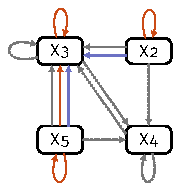
\includegraphics[width=4.5cm,keepaspectratio]{fig_dfg}
\caption{\textsc{dfg} of the mwp-matrix}\label{fig:fail-dfg}
\end{subfigure}\hfill%
%! suppress = NoExtension
\begin{subfigure}{.45\textwidth}
\centering
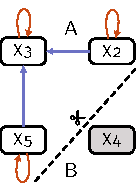
\includegraphics[width=3.2cm,keepaspectratio]{fig_cut.pdf}
\caption{Grouping and independence}\label{fig:group-part}
\end{subfigure} \\[1em]
\begin{subfigure}{\textwidth}{
\centering
\begin{minipage}{.35\textwidth}
\begin{implisting}*[label={lst:p1}]
while(*) {
  X3=X2*X2;
  X3=X3+X5; }
\end{implisting}
\end{minipage}%
\hspace{2em}%
\begin{minipage}{.35\textwidth}
\begin{implisting}*[label={lst:p2}]
while(*) {
  X4=X4+X5;
}
\end{implisting}
\end{minipage}
\caption{Sub-programs}\label{lst:sub-progs}
}\end{subfigure}
\caption[A demonstration of improved derivation failure handling]{
A demonstration of improved \ndx{derivation failure} handling. The program
(\ref{lst:whole-p}) is a modified version of \exname. The variable \pr|X4|
causes failure in every derivation (\ref{fig:fail-matrix}). Starting
with~\ref{fig:fail-dfg}, we restrict the graph to derivations where non-failing
variables can be bounded. This reduces the edges to those shown
in~\ref{fig:group-part}. The sub-program that corresponds to variables in set
\(\mathsf{A}\) (\ref{lst:sub-progs}, above) is derivable.\index{derivability}
}\label{fig:part-prog}
\end{figure}

\begin{example}[Evaluating an always failing derivation]\label{ex:whl}
The program in~\autoref{lst:whole-p} is not derivable because variable \pr|X4|
fails in every derivation.\index{derivation failure} The area of failure, that
we want to isolate, is shaded in the \ndx{mwp-matrix}
of~\autoref{fig:fail-matrix}. Not all variables are problematic. There is no
dependency from \pr|X4| to variables \pr|X2| and \pr|X5| (row \pr|X4|). Variable
\pr|X3| is more complicated due to the ∞\symbo{infty} coefficients\index{flow
coefficient} in column \pr|X3|. Since we want derivations where \pr|X3| is
derivable\index{derivability}, we compute its \ndx{choice vector}: \(\big(\{2\},
\{0,1,2\}\big)\). At index 0, variable \pr|X3| permits one \ndx{derivation
choice}: 2. Applying \((2,0)\) to the \ndx{mwp-matrix}, at column \pr|X3|,
yields coefficients: \(\text{\pr|X2|} \mapsto w\), \(\text{\pr|X3|} \mapsto m\),
\(\text{\pr|X4|} \mapsto 0\), and \(\text{\pr|X5|} \mapsto w\)\symbo{map}. The
\(0\)\symbo{zero} reveals that in every derivable case variable \pr|X3| is
independent of \pr|X4|. Therefore, variables \pr|X3|, \pr|X2| and \pr|X5| can be
assigned \ndx{mwp-bound}s.
\end{example}

\subparagraph*{Variable grouping} (\autoref{fig:group-part}).
The whole-program derivability is first determined by~\autoref{subsec:eval}. In
the negative case, at least one variable must be failing. Crucially, a failing
variable fails in every derivation. Therefore, it suffices to evaluate variables
individually for at most \(p\)\symbo{p} coefficients\index{flow coefficient},
by~\autoref{alg:algo}. We group variables into two sets. Set \(\mathsf{A}\) with
variables that satisfy polynomial value growth, and set \(\mathsf{B}\) with
variables that fail. Which set each variable belongs to is determined by the
existence of a \ndx{choice vector}.

\subparagraph*{Establishing independence from failure} (\autoref{fig:group-part}).
Recall, the \(0\)\symbo{zero} coefficients\index{flow coefficient} track
{absence} of data flows between variables. Thus, we can determine if sets
\(\mathsf{A}\) and \(\mathsf{B}\) are data-flow independent\index{data flow
independence} from the \(0\)s. We must ensure that there is no data flow
\emph{from} the failure set \(\mathsf{B}\) to set \(\mathsf{A}\) in the cases
where variables in \(\mathsf{A}\) are derivable. The condition can be determined
by direct inspection of the \ndx{mwp-matrix}. The independence condition
corresponds to a cut of the \ndx{data flow graph}.

\subparagraph*{Partitioning to sub-programs} (\autoref{lst:sub-progs}).
When failure independence is affirmative, we {partition} the whole-program into
two sub-programs.\footnote{This is a conceptual step; no concrete program
transformation is necessary.} These sub-programs correspond to the data flows in
sets \(\mathsf{A}\) and \(\mathsf{B}\). No bound can be derived for the failing
variables in set \(\mathsf{B}\). Variables in set \(\mathsf{A}\) are analyzed by
the standard rules of the flow calculus\index{mwp-calculus}, which ensures
\ndx{soundness}. \emph{Derivability of this sub-program is the source of
increase in the flow calculus expressivity.}\index{expressiveness}

\subsection{mwp-bounds as Postconditions}
\label{sec:pc-analysis}

\subsubsection{Optimal mwp-bounds by form}
\label{subsec:categories}

The enhanced flow calculus\index{mwp-calculus} now provides a technique for
\ndx{postcondition} inference. We aim to compute the optimal postconditions for
each variable, if they exist. There are two unresolved concerns. First,
\ndx{mwp-bound}s cannot be totally ordered since some forms are incomparable.
Second, mwp-bounds of different form can evaluate to the same numeric
polynomial. For example, the three mwp-bounds \(W_1 \equiv
\max(0,\prm{X1}+\prm{X2})+0\)\symbo{bound}\symbo{xvar} and \(W_2 \equiv
\max(\prm{X1},0)+\prm{X2}\) and \(W_3 \equiv \max(\prm{X2},0)+\prm{X1}\) are all
numerically equal to \(\prm{X1}+\prm{X2}\). Therefore, reasoning about
optimality requires an alternative approach.

To establish an ordering, we leverage two built-in features of the flow
calculus. The individual coefficient are ordered \(0 < m < w < p <
\infty\)\symbo{zero}\symbo{m}\symbo{w}\symbo{p}\symbo{infty}. Moreover, the
mwp-bounds carry semantic meaning \emph{by form}. The growth of a variable value
is at most {linear} (\resp iteration-independent, iteration-dependent) if its
\ndx{mwp-bound} contains at most \(m\) (\resp \(w\), \(p\))
coefficients.\index{flow coefficient} This gives sufficient justification for
our definition of optimality.

\begin{definition}[Optimality]
We define an order on mwp-bounds by form, by the \emph{maximal} coefficient it
contains: \(0 < m\text{-bound} < w\text{-bound} < p\text{-bound} < \infty
\text{(none)}\). A variable's mwp-bound is optimal\index{mwp-bound!optimal} if
it is the least bound in this order.
\end{definition}

\noindent For example, among \(W_1, W_2\), and \(W_3\)\symbo{bound}, the
\(w\)-bound\symbo{w} \(\max(0,\prm{X1}+\prm{X2})+0\) is optimal because it
contains no \(p\)\symbo{p} coefficients.\index{flow coefficient} It supplies the
evidence that the variable's value growth is eventually loop iteration
independent (discussed in~\autoref{subsec:disclaimer}). The other candidates
\(W_2\) and \(W_3\) are too weak to reach the same conclusion. Finding a single
derivation that admits the optimal form is sufficient.

\subsubsection{Variable postcondition search}
\label{subsec:pc-search}

When a program is derivable, or a variable is disjoint from failure, the general
procedure for deriving a variable's optimal \ndx{postcondition} is as follows.

\begin{enumerate}
\item
Run the \ndx{mwp-matrix} evaluation (\autoref{alg:algo}) iteratively. Construct
the set \(\mathcal{S}\)\symbo{dset} from \ndx{monomial}s whose \ndx{flow
coefficient} is greater than \(m\)\symbo{m} (next \(w\)\symbo{w}, then
\(p\)\symbo{p}).
\item Stop at the first \ndx{choice vector}.
This solution is optimal.
\end{enumerate}

\noindent
Since the search focuses on individual variables, we may want to ask whether
multiple \ndx{postcondition}s can occur concurrently. To determine the answer,
we take the intersection of their \ndx{choice vector}s
(\autoref{def:intersect}). A non-empty intersection specifies the derivations in
which both \ndx{postcondition}s hold. Related questions about
\ndx{postcondition}s can be formulated similarly, as operations on \ndx{choice
vector}s.

\begin{definition}[Choice vector intersection]
\label{def:intersect}\index{choice vector}
Letting \(\vec{C_a} = (a_1, a_2,\dots,a_k) \)\symbo{cv} and \(\vec{C_b} =
(b_1\), \(b_2\), \(\dots\), \(b_k)\) be \ndx{choice vector}s of length
\(k\)\symbo{k2}, we define the intersection of \(\vec{C_a} \text{ and }
\vec{C_b} \) as \[ \vec{C_a} \cap \vec{C_b} = \begin{cases} (a_1 \cap b_1, a_2
\cap b_2, \dots, a_k \cap b_k), & \text{ if } \not\exists i \text{ such that }
a_i \cap b_i = \emptyset, \\ \emptyset, & \text{ otherwise.}\end{cases}
\]%\qedhere
\end{definition}

\begin{example}
[Successful and optimal postcondition of \texttt{X3}]
\label{ex:opt-derivation}
By \autoref{ex:derivable}, \exname is derivable\index{derivability} by
\ndx{choice vector} \(\big(\{0, 1, 2\}, \{0\}\big)\). By \autoref{ex:wbound},
variable \pr|X3| is assigned its optimal postcondition in derivations
\(\big(\{2\}, \{0,1,2\}\big)\). The whole-program is derivable \emph{and}
variable \pr|X3| is assigned its optimal \ndx{postcondition} in derivations
defined by choices \( \big(\{0, 1, 2\}, \{0\}\big) \cap \big(\{2\},
\{0,1,2\}\big) = \big( \{2\}, \{0\}\big) \).
\end{example}

\subsubsection{Program analysis for postcondition inference}
\label{subsec:inference}

Postcondition\index{postcondition} inference requires adjusting the imperative
language\index{imperative programs} (\autoref{subsec:imp-language}) to a
language of loops. A \emph{loop program} starts with a looping command
(\pr|while| or \pr|loop|) whose body\index{loop body} is any command in the
imperative language. Using the \ndx{mwp-matrix} evaluation procedure, we compute
\ndx{postcondition}s for all variables that have expressible \ndx{mwp-bound}s.
To avoid repeated analysis, we proceed from loop nests\index{nested loop} to
parent and compose mwp-matrices\index{mwp-matrix} in a bottom-up manner.
Postcondition\index{postcondition} inference of loop
\(\mathcal{C}\)\symbo{prog2} is defined as follows.

\begin{enumerate}
\item Extract all (possibly nested)\index{nested loop} loops from the
program \(\mathcal{C}\)\symbo{prog2}.
\item (bottom-up) For each loop \(l\):\symbo{loop}
\begin{enumerate}[label=(\roman*)]
\item Run the mwp analysis to derive the \ndx{mwp-matrix}, \(l :
M\).\symbo{matrix}\symbo{loop}
\item Using \autoref{alg:algo}, evaluate \(M\)\symbo{matrix} to determine if
\(l\) is derivable.\index{derivability}
%! suppress = MissingImport
\begin{itemize}
    \item[] \(\triangleright\) If yes: mark every variable as satisfactory.
    \item[] \(\triangleright\) If no: mark the non-failing variables as
    satisfactory (\autoref{subsec:bounds-at-failure}).
\end{itemize}
\item Evaluate satisfactory variables for optimal \ndx{postcondition}s
(\autoref{subsec:pc-search}).
\item Record the postconditions of satisfactory variables.
\end{enumerate}
\item Return the analysis result for \(\mathcal{C}\)\symbo{prog2}.
\end{enumerate}

\subsubsection{Postcondition categories as descriptors of variable value
behavior}
\label{subsec:disclaimer}

A language of loops restricts the kind of computations we may encounter. The
inferred \ndx{postcondition}s can be described by the following categories.

\begin{description}

\item[Linear.]\index{mwp-bound!linear}
A variable's \ndx{mwp-bound} is linear if its value does not change or it is
a target of direct assignment (without arithmetic). Inside loops, other
operations are \enquote{too strong} to retain linear behavior. In \exname,
variables \pr|X1|, \pr|X2| and \pr|X5| are linear because their values never
change.

\item[Iteration-independent.]\index{mwp-bound!iteration-independent}
A variable is iteration-independent if its final value depends on a fixed
number of iterations (\eg the first or last one) or eventually reaches a
fixed point. Iteration independence\index{iteration independence} means
that, beyond the fixed point, the variable is unaffected by an increase in
loop iteration count.\index{iteration space} Thus, iteration-independence is
a quasi-invariance\index{quasi-invariant} property. In \exname, if the loop
iterates at least once, the final value of \pr|X3| is determined by \pr|X2|
and \pr|X5|.

\item[Iteration-dependent.]\index{mwp-bound!iteration-dependent}
Arithmetic computations involving multiple changing variables lead to
iteration-dependent value growth.\index{iteration dependence} It may occur
in \ndx{bounded loop}s, but not otherwise. This is because a continuously
increasing value may be boundable under finite iteration, but not if the
loop is unbounded\index{unbounded loop}. In \explain, changing the number of
times the loop iterates changes the final value of \pr|X4| respectively.
This makes \pr|X4| iteration-dependent.

\item[Inconclusive.]
If no expressible \ndx{postcondition} exists, the variable is inconclusive.
It characterizes cases where a variable's value growth is outside the
previous three categories. In~\autoref{ex:whl}, since the loop does not
terminate, the value of \pr|X4| grows in perpetuity. This makes the
variable's value growth inconclusive.

\end{description}

\paragraph*{A note on numerical minimality}
One variable may be assigned multiple incomparable \ndx{mwp-bound}s. The
definition of optimality\index{mwp-bound!optimal} does not guarantee the
selected \ndx{postcondition} is the numerical minimum by evaluation. For
example, variable \pr|X3| in \exname is assigned three mwp-bounds \(W_1 \equiv
\max(\prm{X3},\prm{X2})+\prm{X1} \times \prm{X5} \) and \(W_2 \equiv
\max(\prm{X3},\prm{X2}+\prm{X5}) \) and \(W_3 \equiv
\max(\prm{X3},\prm{X5})+\prm{X1} \times \prm{X2} \).\symbo{bound}\symbo{equiv}
For purpose of this example, assume \(\prm{X1}>0\) to consider the iterative
case and ignore \(W_2\).\symbo{bound} This leaves two alternatives. These can
evaluate to distinct numeric values, yet both are equally optimal by
definition.\index{mwp-bounds!optimal}

\subsubsection{Implementing postcondition inference with \impl}
\label{subsec:implementation}

We implemented the analysis of~\autoref{subsec:inference} as an extension of the
static analyzer \ndx{pymwp}. \ndx{pymwp}~\cite{aubert2023b} is an open source
implementation of the flow calculus of mwp-bounds \index{mwp-calculus} on a
subset of \pr|C|.\index{C} \ndx{pymwp} takes as input a \pr|C| file and analyzes
variable value growth in each of its functions. Our implementation adds to
\ndx{pymwp} a new loop analysis mode, \ndx{\impl}. The loop analysis is
complementary to the default function analysis mode, which we name \ndx{\impf}
for distinction. The primary differences are that \ndx{\impl} looks for
{optimal} bounds\index{mwp-bound!optimal} by variable in a {loop}, and
\ndx{\impf} finds existence of {any} bound for all variables in a {function}.
Though applicable to both, the paper enhancements are implemented only in
\ndx{\impl} to enable evaluation.

During program analysis, the input file is mapped to the imperative language
of~\autoref{def:lang}.\index{imperative programs} Only loops that are fully
expressible in the imperative language are analyzed. Analyzing program fragments
is possible due to \ndx{compositionality} of the flow
calculus.\index{mwp-calculus} Stated differently, we can apply the analysis
early, even if some program parts are missing. \ndx{pymwp} supports all loop
constructs of \pr|C|.\index{C} The flow calculus treats the \ndx{iteration
space} conservatively as an over-approximation. Keywords \pr|break| and
\pr|continue| have no observable impact. Similarly, verification macros like
\pr|assert|\index{assertion} may be present, but they do not impact the
analysis.

When a \pr|C|\index{C} loop construct is obviously bounded\footnote{For example,
in \pr|for(int i=0;i<N;i++)| the iterator \pr|i|\index{iteration variable} must
not occur in the body and the body operations are arithmetic. Without nesting,
it is clearly a finite loop.}, it is treated as a \ndx{bounded loop} in the flow
calculus.\index{mwp-calculus} Otherwise, the construct is treated as an
\ndx{unbounded loop}. Detection of \ndx{loop boundedness} impacts the number of
derivable\index{derivability} variables, since a \ndx{bounded loop} permits
iteration-dependency.\index{mwp-bound!iteration-dependent} The current detection
is based on loop form and it is still rudimentary. In the future, improving the
analyzer's handling of richer loop forms would yield more bounded variables.

To use the analysis results as concrete verification \ndx{assertion}s, two more
steps are required. First, we must record the initial variable values because
they are needed to express \ndx{postcondition}s. Next, we must complete the
parts that are left implicit in \ndx{mwp-bound}s, like constants.
\autoref{app:sec:verified} demonstrates how we perform both steps. In general,
the \ndx{postcondition}s provide bounding expressions \wrt input variables, with
some possible omissions. However, filling in the expression is easier than
starting with no expression at all.

\subsection{Comparing Related Techniques}
\label{sec:related-works}

\subsubsection{Automatic inference of specification conditions}
\label{subsec:automatic-inference}

Our work relates primarily to approaches that aim to unify software verification
and complexity. Whereas \ndx{loop invariant}s are used in~\cite{nguyen2017} to
obtain complexity results, we synthesize specification conditions starting from
\ndx{complexity analysis}. The bidirectionality suggests that further
investigations that connect the two topics is warranted. Narrowing down to
\ndx{specifications}, automatic specification inference in general is a
challenging problem~\cite{dillig2013,yu2023}. It is common to break down the
problem into smaller parts: \ndx{precondition}s, \ndx{postcondition}s, and
(inductive)\index{invariant!inductive} \ndx{invariant}s. Inference of
\ndx{postcondition}s is the most relevant to our analysis. Although
\ndx{invariant inference} is studied extensively in
literature~\cite{karr1976,cousot1978,colon2003,sankaranarayanan2004,dillig2013,si2018,ryan2020,yao2020,yu2023,nguyen2014,nguyen2017},
existing works that intentionally target \ndx{postcondition}s are
rare~\cite{popeea2006,molina2021}.

There are a few instances that infer \ndx{postcondition}s statically.
In~\cite{popeea2006}, show how \ndx{abstract interpretation} can be used to
obtain a static technique for \ndx{postcondition} inference. Conceptually it is
close to our goals, but \ndx{abstract interpretation} differs considerably from
the flow calculus.\index{mwp-calculus} Moreover, no implementation is available
for comparison. The complexity analyzer \ndx{KoAT}~\cite{giesl2022} is a static
analyzer with an open source implementation. However, it targets
complexity-theoretic program properties, like time and \ndx{size bound}s, and is
not specialized in verification.

Dynamic analyzers are complementary to static techniques.\index{dynamic program
analysis} They inspect \ndx{program trace}s to infer \emph{likely}
invariants\index{likely invariant} at the traced program points.
\ndx{EvoSpex}~\cite{molina2021} is a dynamic postcondition analyzer. It is
designed for \ndx{Java} methods for reasoning about \ndx{postcondition}s in
classes (accessors, mutators, heap structures, \etc); and thus distant from
numerical loop\index{numerical loops} analysis. The \ndx{invariant} detector
\ndx{Daikon}~\cite{ernst2007} handles many program constructs, including
\ndx{numerical loops}. Since \ndx{Daikon} is compatible with our problem
formulation, we discuss it in~\autoref{subsec:comparison}).
\ndx{DIG}~\cite{nguyen2014} is another dynamic numeric \ndx{invariant}
generator. \ndx{DIG} can perform \ndx{invariant inference} at arbitrary program
points, which makes it usable as a \ndx{postcondition} detector. Although it is
similar to \ndx{Daikon}, \ndx{DIG} mixes static and dynamic techniques to obtain
more informative results. In general, \ndx{dynamic program analysis} differs
notably from \ndx{static program analysis}. Since the results are based on
traces\index{program trace}, they are necessarily
incomplete.\index{incompleteness} The quality of inferred results is directly
related to the available analysis inputs. Importantly, a dynamic analyzer
requires executing the input program, which implies that the program must be
runnable. The same is not necessary for our analysis that can work with program
fragments.

\subsubsection{A Comparison of Alternative Approaches}
\label{subsec:comparison}

Since we aim to support concrete verification tasks, we must compare our
analysis to available implementations that can address the same problem. In this
section, we compare\footnote{Refer to \autoref{app:sec:comparison} for the
technical details of this comparison.} \ndx{\impl} to three mature\footnote{Each
analyzer is developmentally stable with 10+ years of history.} analyzers:
\ndx{KoAT}, \ndx{Duet}, and \ndx{Daikon}. These analyzers are designed for
\ndx{complexity analysis}, verification, and \ndx{invariant inference}, \resp
Each analyzer analyzes different program scopes (\cf~\autoref{tab:summary}
and~\autoref{subsec:analyzer-scopes}) and has a different specification of
output format. Therefore, a statistical comparison is insufficient for useful
comparison. A better way is to present canonical cases that the analyzers handle
differently. As comparison workloads we consider the loops
of~\autoref{fig:loops}. They are instances from the benchmarks used
in~\autoref{sec:performance}. To give a preview of our findings---which we
summarize in~\autoref{tab:summary}---the alternative analyzers are {orthogonal}.
The comparison shows \ndx{\impl} is useful in cases the other tools ignore, and
vice versa.

\begin{center}
\captionsetup{type=figure}
\begin{minipage}{\textwidth}
\begin{minipage}[t]{.33\textwidth}
\begin{implisting}*[numbers=none]
for(int i=0;i<X1;i++)
{ X3=X2*X2;
  X3=X3+X5;
  X4=X4+X5; }
\end{implisting}
\captionof{lstlisting}[Benchmark: \explain]{\mbox{\explain}}
\label{lst:case-1}
\end{minipage}\hfill%
\begin{minipage}[t]{.33\textwidth}
\begin{implisting}*[numbers=none]
while(nondet())
{ X1=X2+X2;
  X2=X3+X3;
  X4=X5+X5; }
\end{implisting}
\captionof{lstlisting}[Benchmark: Function condition]
{\mbox{Function condition}}
\label{lst:case-2}
\end{minipage}\hfill%
\begin{minipage}[t]{.3\textwidth}
\begin{implisting}*[numbers=none]
assume(y==0);
while(y<1000)
{ x=x+y;
  y=y+1; }
\end{implisting}
\captionof{lstlisting}[Benchmark: Finite iteration]
{\mbox{Finite iteration}}
\label{lst:case-3}
\end{minipage}
\captionof{figure}[Loop cases for analyzer comparison]{
Loop cases for analyzer comparison. The loop in~\ref{lst:case-1} is known to
terminate\index{termination} and its \ndx{guard variable} \pr|X1| does not occur
in the body. In~\ref{lst:case-2}, the loop \ndx{iteration space} and
\ndx{termination} are unknown since they are controlled by a nondeterministic
function\index{nondeterminism}. The loop in~\ref{lst:case-3} has a fixed
\ndx{iteration space}, but the \ndx{postcondition} of \pr|x|\symbo{xvar} is
difficult to infer. Assuming \(\prm{y}=0\), the precise formula is \(\prm{x'} =
\prm{x} + (\prm{y'} \times \prm{y'} - \prm{y'})\symbo{xvar}\symbo{Xprime} \div
2\) where \pr|y'| is iteration count.
}\label{fig:loops}
\end{minipage}
\end{center}

\paragraph*{Inference with \impl}
The results of \ndx{\impl} give a baseline for comparison.

\begin{itemize}

\item \autoref{lst:case-1}: As explained in~\autoref{subsec:overview}.

\item \autoref{lst:case-2}: \pr|X3| and \pr|X5| are linear.
The other are
\(\prm{X2'}\leq\max(\prm{X2},\prm{X3})\),
\( \prm{X4'}\leq\max(\prm{X4},\prm{X5})\), and
\(\prm{X1'}\leq\max(\prm{X1},\prm{X2}+\prm{X3})\).\symbo{Xprime}

\item \autoref{lst:case-3}: The program converts to a \ndx{bounded loop}. The
constants \pr|1| and \pr|1000| are lifted to inputs \(\prm{c}_1\) and
\(\prm{c}_2\), \resp The \ndx{postcondition}s are
\(\prm{x'}\leq\prm{x}+\prm{c}_2\times(\prm{c}_1 + \prm{y})\) and
\(\prm{y'}\leq\prm{y}+(\prm{c}_1\times\prm{c}_2)\).

\end{itemize}

\paragraph*{Complexity analyzer KoAT}
\ndx{KoAT}~\cite{koat} is a part of the automated \ndx{termination} and
complexity prover \ndx{AProVE}~\cite{giesl2016}. \ndx{KoAT} infers complexity
bounds:\index{asymptotic bounds} time, cost, \ndx{size bound}s, \etc The bound
most relevant to our problem is the \emph{\ndx{size bound}}, which indicate how
large the absolute value of an integer variable may become~\cite{lommen2023}.
Applying \ndx{KoAT} on \ndx{C} programs requires compiling the C code (through
\ndx{LLVM bitcode}) into an \ndx{integer program}. The transformed program is
then analyzed by \ndx{KoAT}~\cite{giesl2022}. The translation step renames the
program variables. Variables that do not contribute to the complexity result are
discarded during pre-processing. This treatment has the following effects: (i)
\ndx{KoAT} can distinguish between loops that differ only on iteration counts,
and (ii) \ndx{size bound}s are inferred only for variables that impact the loop
iteration. The latter is the complement of the flow
calculus,\index{mwp-calculus} where the iterator of a \ndx{bounded loop} is not
allowed to occur in the body.\index{loop body}

\begin{itemize}
\item~\autoref{lst:case-1}: We obtain \(\prm{X1'} : 2 \cdot \prm{X1}\) and
\(\prm{i'}: \prm{X1}+ 2\); and \pr|X2|--\pr|X5| are discarded.

\item~\autoref{lst:case-2}: No \ndx{size bound}s are generated for variables
\pr|X1|--\pr|X5|.

\item~\autoref{lst:case-3}: Variable \pr|y| has precise \ndx{size bound}
\(\prm{y}: 1000\). Variable \pr|x| is discarded.
\end{itemize}

\paragraph*{Duet -- the analyzer of unbounded concurrency}
\ndx{Duet} is a static verifier for \ndx{concurrent programs} whose \ndx{thread}
count cannot be statically bounded~\cite{duet}. We include it in this comparison
because it contains analysis techniques that relate to our problem. In
particular, the implementation of {\ndx{transition ideal}s}~\cite{cyphert2024}
computes {loop summaries} that produce over-approximations of a formula that
describes the loop body. The summaries can capture non-linear
invariants\index{invariant!non-linear} and generalize over arbitrary control
flow. The theory of transition ideals is monotone. In other words, a program
with more precise \ndx{specifications} yields a more informative loop summary.
Then, \ndx{Duet} aims to prove program correctness using the \ndx{invariant}s
generated from \ndx{transition ideal}s.

\begin{itemize}
\item Listings~\ref{lst:case-1} --~\ref{lst:case-3}:
    In absence of \ndx{assertion}s, \ndx{Duet} produces a
    single response, \pr|no errors and no unsafe assertions|. This response is
    not meaningful for our use case. After adding \ndx{postcondition}s
    (\ndx{assertion}s) manually, \ndx{Duet} verifies them
    successfully. For example, if we add to~\autoref{lst:case-3} the
    \ndx{assertion}s
    \(\prm{x'}=\prm{x}+(\prm{y'}\times\prm{y'}-\prm{y'}) \div 2 \) and
    \(\prm{y'}=1000 \), \ndx{Duet} verifies the program with \pr|0 errors,|
    \pr|2 safe assertions|. When \ndx{assertion}s are not
    available, \ndx{\impl} could assist \ndx{Duet} toward obtaining the initial
    assertions.
\end{itemize}

\paragraph*{Postconditions with Daikon}
\ndx{Daikon}~\cite{ernst2007,daikon} is a dynamic\index{dynamic program analysis}
\ndx{invariant} detector with front-ends to support many programming languages.
\ndx{Daikon} predicts \ndx{likely invariant}s at function entry and exit points.
Critically, the function internals are opaque during \ndx{invariant} detection.
The inference relies on execution traces\index{program trace}, \ndx{invariant
template}s, and configuration options. \ndx{Daikon} infers \ndx{postcondition}s
for a \pr|return| variable and a single function may generate multiple
\ndx{postcondition}s. Since the \ndx{invariant}s are likely, they must be
checked for correctness, possibly manually. \ndx{Daikon} does not produce
results for the displayed fragments, but after a modification to a
whole-program, it infers the following.

\begin{itemize}

\item~\autoref{lst:case-1}: \(\prm{X3'} > \prm{X2}\), \(\prm{X3'} > \prm{X4}\)
and \(\prm{X3'} > \prm{X5}\).\symbo{Xprime} These either do not generalize or
require additional \ndx{assumption}s to prove.

\item~\autoref{lst:case-2}: No result.

\item~\autoref{lst:case-3}: Precise numeric value of \pr|x| or \pr|y|, depending
on which one is returned. Although the arithmetic formula is not recovered,
\ndx{Daikon} is the only technique that can give a precise value for \pr|x|.

\end{itemize}

\begin{table}[h]
\begin{tabularx}{\textwidth}{@{}X@{}cccc@{}}
\toprule
\textbf{Feature}         &
\textbf{\ndx{Daikon}}          &
\textbf{\ndx{Duet}}            &
\textbf{\ndx{KoAT}}            &
\textbf{\ndx{\impl}}           \\
\midrule
Analysis scope                & function entry/exit   & \ndx{invariant}s     & loop control         & \ndx{loop body}     \\
(\autoref{subsec:analyzer-scopes}) \\
Input format                  & execution traces\index{program trace}        & program              & program              & program       \\
Output format                 & \ndx{likely invariant}s     & SAT/error      & \ndx{size bound}s    & \ndx{mwp-bound}s    \\
Numerical domain              & \(\mathbb{Z}\)        & \(\mathbb{Z}\)       & \(\mathbb{Z}\)       & \(\mathbb{N}\) \\
Postcondition expressivity    & >+                    & >+                   & >+                   & +             \\
Program fragment analysis     & \snone                & \spart               & \sfull               & \sfull        \\
Handles program divergence    & \snone                & \sfull               & \sfull               & \sfull        \\
Distinguishes iteration count & \sfull                & \snone               & \sfull               & \snone        \\
Body variables coverage       & \spart                & \sfull               & \spart               & \sfull        \\
Results soundness             & \snone                & \sfull               & \sfull               & \sfull        \\
Postconditions for
\autoref{fig:loops}           & \spart \snone \spart  & \snone \snone \snone & \spart \snone \spart & \sfull \sfull \sfull \\
\bottomrule
\end{tabularx}\symbo{nat}
\caption[Summary of analyzer capabilities, behaviors, and assumptions]{
Summary of analyzer capabilities, behaviors, and assumptions. For input
format, we write \emph{program} to mean syntactical analysis written in a
subset of the \ndx{C} language, though the subsets differ. A positive
response is phrased as favorable: \mbox{\sfull = yes}, \mbox{\spart =
partial}, \mbox{\snone = no}.
}\label{tab:summary}
\end{table}

\subsection{Experimental Evaluation}
\label{sec:performance}

We examine two questions about the implementation of our technique.

\begin{enumerate}

\item \textbf{How effective is \ndx{\impl} at discovering
\ndx{postcondition}s in general?}
We execute \ndx{\impl} against four benchmark suites that include a rich set
of benchmarks from \ndx{complexity theory} to loop\index{loop invariant}
\ndx{invariant inference}. Three of the suites are design-independent of the
applied analysis technique.

\item \textbf{What is the concrete impact of the new theoretical
enhancements?}
We hypothesize that the introduced enhancements are critical for extending
the utility of the flow calculus.\index{mwp-calculus} To quantify this
improvement, we compare performance of \ndx{\impl} and \ndx{\impf} across
the four benchmark suites.

\end{enumerate}

\paragraph*{Setup: benchmarks, metrics, and environment}
\label{subsec:exp-setup}
We consider four benchmark suites, of numerical \ndx{C} loops\index{numerical
loops}, and 620 total problem (detailed in~\autoref{app:subsec:bench}). The
{complexity} suite is mainly linear time complexity problems whose
\ndx{termination} behavior is unknown. The
{linear}~\cite{si2018}\index{invariant!linear} and
{non-linear}~\cite{nguyen2017,yu2023}\index{invariant!non-linear} suites come
from loop\index{loop invariant} \ndx{invariant inference} literature. The
non-linear suite includes classic numerical algorithms like geometric series and
divisor computations. The {mwp} suite~\cite{aubert2023b} problems are designed
pose challenges to analyses based on the flow calculus of
mwp-bounds.\index{mwp-calculus} All suites include branching statements and
nondeterministic\index{nondeterminism} control expressions that simulate
external function calls. The complexity and non-linear suites have problems with
sequential and \ndx{nested loop}s. As evaluation metrics, we recorded the count
and kind of obtained \ndx{postcondition}s (\ie \ndx{mwp-bound}s). We also
recorded all meta-data collected by \ndx{pymwp} like program statistics. We set
the timeout to 10 seconds. Without timeouts the metrics are deterministic. We
ran all experiments on commodity hardware; on a native 10-core macOS 15.3.2 M1
arm64 host with 16 GB of RAM\@. All experiment results are in
\autoref{tab:results}.

\begin{table}[h]
\begin{tabularx}{\textwidth}{@{}lXrcr@{\hspace{1em}}r@{\hspace{1em}}r@{\hspace{1em}}r@{\hspace{1em}}r@{}}
\toprule
\textbf{Analyzer}
& \multicolumn{1}{l}{\textbf{Suite}}
& \multicolumn{1}{c}{\textbf{Loops}}
& \textbf{Variables}
& \multicolumn{1}{c}{\textbf{Bounds}}
& \textbf{m}
& \textbf{w}
& \textbf{p}
& \multicolumn{1}{c}{{\({\infty}\)}}
\\
\midrule
\impl   & Complexity  & 623 (.84)   & 1407   &   988 (.70) &   567 & 49 & 372 & 419 (.30) \\ %&  43158 & (58.32)  \\
(ours)  & Linear      & 49  (1.0)   & 103    &    80 (.78) &    22 &  7 &  51 &  23 (.22) \\ %&    299 &  (6.10)  \\
& Non-linear  & 43  (.90)   & 172    &   107 (.62) &    48 &  8 &  51 &  65 (.38) \\ %&    461 &  (9.60)  \\
& mwp         & 30  (1.0)   & 105    &    77 (.73) &    38 & 30 &   9 &  28 (.27) \\ %&   2666 & (88.87)  \\
\midrule
& \multicolumn{1}{l}{\textbf{Suite}}
& \multicolumn{1}{c}{\textbf{Functions}}
& \textbf{Variables}
& \multicolumn{1}{c}{\textbf{Bounds}}
& \textbf{m}
& \textbf{w}
& \textbf{p}
& \multicolumn{1}{c}{{\({\infty}\)}}
\\
\midrule
\ndx{\impf}    & Complexity  & 399 (.79)   &  1153  & 616 (.53)  & 330 &  6 & 280 & 537 (.47) \\ %&   18674 & (37.05) \\
(prior)  & Linear      &  49 (1.0)   &   131   & 95 (.73)  &  38 &  1 &  57 &  36 (.27) \\ %&     117 &  (2.39) \\
& Non-linear  &  29 (.78)   &   159   & 60 (.38)  &  14 &  3 &  43 &  99 (.62) \\ %&     744 & (20.11) \\
& mwp 	      &  30 (1.0)   &   105   & 66 (.63)  &  28 & 22 &  16 &  39 (.37) \\ %&    1878 & (62.60) \\
\bottomrule
\end{tabularx}
\caption[Experiment results for \impf and \impl]{
Experiment results for \ndx{\impf} and \ndx{\impl} with totals and (mean).
\emph{Loops}/\emph{functions} shows the number of analyzed instances and suite
coverage (\%). \emph{Bounds} is the number of inferred \ndx{postcondition}s,
with the mean is relative to analyzed \emph{variables}. The \emph{mwp}-columns
show a breakdown of postconditions by bound form. The number of unbounded
variables is shown in column \(\infty\).
}\label{tab:results}
\end{table}

\subsubsection{Inference generalizability}
\label{subsec:rq1-res}

Across the four suites, \ndx{\impl} succeeds at analyzing 84\%-100\% of the
loops. It finds \ndx{postcondition}s for 62\%-78\% of variables occurring in
those loops. The \ndx{postcondition}s are different in form from most complexity
analyzers (refer to~\cite{lommen2023,aubert2023b}). Most complexity analyzers
are essentially restricted to linear arithmetic~\cite{lommen2023}.
Encouragingly, \ndx{\impl} shows success also on the non-linear suite. The
results are positive because the suite contains complex arithmetic and natural
algorithms. The linear suite expectedly yields more \ndx{postcondition}s, since
the suite is easier. On the complexity problems, that dominate in problem
quantity, \ndx{\impl} already bounds 70\% of variables. The number depends
largely on how loop boundedness is decided. We expect that, after improving the
current mechanism, \ndx{\impl} would produce even more \ndx{postcondition}s.

We observe some limitations \wrt expressivity.\index{expressiveness} First,
loops with unsupported syntax are not analyzed. For example, some variables in
the complexity suite are updated by a random integer
generator.\index{randomness} Such operations are inherently outside the
guarantees that can be provided by the flow calculus.\index{mwp-calculus} When
the growth rate of some variables is truly beyond polynomial, it is not
expressible as \ndx{mwp-bound}s. Finally, sometimes the polynomial describing
the variable value growth may be too complicated to express. Based on the
findings, further increase in expressivity should be one of the main directions
of future research.\index{expressiveness} In summary, \ndx{\impl} succeeds at
analyzing most loops, and it generates \ndx{postcondition}s for most variables
in those loops.

\subsubsection{Impact of theoretical enhancements}\label{subsec:rq2-res}

We compare \ndx{\impl} and \ndx{\impf} to quantify the impact of the
enhancements introduced in this paper. As practical implementations of the flow
calculus,\index{mwp-calculus} \ndx{\impf} represents the state-of-the-art in the
analysis capabilities. Since the two analysis modes differ on program scopes,
not all results are comparable. However, we pre-processed the mwp-suite such
that it is fully comparable. The mwp-suite results confirm that the paper
enhancements improve abilities to infer \ndx{postcondition}s. On the mwp suite,
\ndx{\impl} bounds 73\% of variables compared to 63\% by \ndx{\impf}. Further,
\ndx{\impl} finds optimal\index{mwp-bound!optimal} bounds, which is reflected in
the distribution of bound forms. The other suites are comparable through the
statistical means. Particularly on the non-linear suite, \ndx{\impf} finds a
bound for only 38\% variables. This is because one failing variable causes
failure of all variables. On the same suite, \impl bounds 62\% variables due to
its enhanced failure handling.

\subsection{Conclusions and Future Directions}
\label{sec:pc-conclusion}

Assistance in specification\index{specifications} inference is paramount to
increase adoption of \ndx{formal methods} in practice. The paper has presented
how to repurpose a complexity-theoretic analysis to \ndx{postcondition}
inference. This required four new enhancements:

\begin{enumerate}[label=(\roman*)]
\item projecting the analysis on individual variables,
\item introducing an evaluation strategy to obtain optimal mwp-bounds,
\item improving derivation failure-handling to increase analysis
\ndx{expressiveness},
\item and adopting the analysis to a new use case, \ie \ndx{formal
verification}.
\end{enumerate}

A comparison study shows our technique offers complementary strengths among the
related inference\index{invariant inference} approaches. The theory is
materialized in an implementation, \ndx{\impl}. Our experiments show that the
paper enhancements improve the flow calculus\index{mwp-calculus} and make it
applicable toward uses in \ndx{formal verification}.

\paragraph*{Future directions}
Although we have extended the flow calculus\index{mwp-calculus} capabilities,
multiple directions for future work remain, and many emerge from this work. The
two main directions concern enriching the analysis \ndx{expressiveness} and
\ndx{precision}. \Eg, leveraging \ndx{assumption}s (if available), tracking
variable immutability, and accounting for control expression would generate more
precise specification conditions. Currently, polynomial \(p\)-flows are not
allowed inside \ndx{unbounded loop}s. Discovering ways to relax this restriction
would improve \ndx{expressiveness} and yield more postconditions. Due to the
complexity-theoretic\index{complexity theory} origins, the flow
calculus\index{mwp-calculus}  targets polynomial \emph{upper} bounds\index{upper
bound}. For verification, it would be useful to extend the technique to also
cover \ndx{lower bound}s, and assign bounds on exponential growth. On the
practical side, our analysis does not cover division operator and requires
expanding operations to binary form. These limitations can be resolved by
refactoring the input program, but should be resolved at the theoretical level.

We are encouraged by the continued enhancements of the flow
calculus\index{mwp-calculus} and discovering its potential uses. The analysis
could already be implemented as a developer plug-in to assist in writing
\ndx{specifications}. In future research, we will consider extending the
capabilities of the flow calculus\index{mwp-calculus}. We are generally curious
about whether similar solver-free syntactic analyses could be designed to infer
\emph{other} specification\index{specifications} conditions. Another ongoing
project is to formally verify\index{formal verification} the flow calculus
theory. The results of this paper provide important justification to the
formalization effort.

\clearpage

\subsection{Appendix A: Application to Program Verification}
\label{app:sec:verified}

The following example shows how to complete an implementation with
specification\index{specifications} conditions, in the verification-aware
\ndx{Dafny} programming language. The \ndx{postcondition}s are those inferred by
our analysis.

\begin{center}
\begin{minipage}{\textwidth}
\captionsetup{type=lstlisting}
\dafnyinputlisting[][]{lucid.dfy}
\captionof{lstlisting}[\exname verified in Dafny]
{\exname verified in \ndx{Dafny}.}
\label{lst:dafny-ex}
\end{minipage}
\end{center}

Concrete program verification requires two additional steps. First, recording
the initial variable values (L4). This is simply a matter of creating copies of
variables. Recording the initial values enables referring to them in the
\ndx{postcondition}s. Second, we add the constants (L14--16) omitted in the
\ndx{postcondition}s of our analysis. Although this step requires manual effort,
is it significantly easier to \enquote{fill in} the constants, than to infer
full \ndx{assertion} clauses. Maintaining human oversight in this step has an
additional benefit. It forces to check that the \ndx{assertion}s are sensible.
If the implementation has a bug---\eg variable grows exponentially when it
should not---the bug becomes detectable during this step. A fully automatic
technique would not alert to the issue.

After adding \ndx{invariant}s, the \ndx{Dafny} verifier immediately constructs a
proof, which confirms that the \ndx{assertion}s always hold. Generating suitable
inductive\index{invariant!inductive} loop \ndx{invariant}s\index{loop invariant}
is a challenge for the related works that specialize in invariant
inference\index{invariant inference}.

\subsection{Appendix B: Technical Details of Analyzer Comparison}
\label{app:sec:comparison}

\subsubsection{Executing the analyzers}\label{subsec:analyzers}

We analyzed the programs in Listings~\ref{lst:ex34}--\ref{lst:l2} as follows.

\paragraph*{$\text{mwp}_\ell$}
We run \ndx{pymwp} v0.6.0 in the loop analysis mode.
\begin{center}
\begin{minipage}{\textwidth}
\captionsetup{type=lstlisting}
\cmdinputlisting[]
[escapeinside=||,emph={pymwp},emphstyle={}]{mwpl.cmd}
\captionof{lstlisting}
[Running pymwp in loop analysis mode]
{Running \ndx{pymwp} in loop analysis mode.}
\label{lst:mwp-bash}
\end{minipage}
\end{center}

\paragraph*{KoAT}
The \ndx{KoAT} web interface is sufficient to confirm our findings.
We applied the following options:
\myok{ }control-flow refinement
\myok{ }\ndx{size bound}s
\myok{ }unsolvable loops, and default timeout.
The web interface address is:

\begin{center}
\href{https://aprove.informatik.rwth-aachen.de/interface/v-koat/c}%
{\pr|https://aprove.informatik.rwth-aachen.de/interface/v-koat/c|}
\end{center}

\paragraph*{Duet}
We ran \ndx{Duet} from source, git revision \pr|1d36b05|, with following
options. The compositional recurrence analysis generates \ndx{invariant}s for
sequential programs. Transition ideals\index{transition ideal} is implemented as
linear and quadratic simulation modes.
\begin{center}
\begin{minipage}{\textwidth}
\captionsetup{type=lstlisting}
\cmdinputlisting[][
    escapeinside=||,alsoletter={.},
    emph={duet\.exe},emphstyle={}]{duet.cmd}
\captionof{lstlisting}[Program analysis with Duet]
{Program analysis with \ndx{Duet}.}
\label{lst:duet-bash}
\end{minipage}
\end{center}

\paragraph*{Daikon}
\ndx{Daikon} requires multiple version of a program, then compiling and tracing
them with \ndx{Kvasir}. The \pr|*| means we trace\index{program trace} multiple
versions of input. \newline

Supply options to \ndx{Kvasir} before the program name argument.

\begin{center}
\begin{minipage}{\textwidth}
\captionsetup{type=lstlisting}
\cmdinputlisting[][escapeinside=||]{dk_trace.cmd}
\captionof{lstlisting}[Creating a trace with Daikon]
{Creating a trace\index{program trace} with \ndx{Daikon}.}
\label{lst:kvasir-bash}
\end{minipage}
\end{center}

After tracing, we run \ndx{Daikon} with following options to infer
\ndx{postcondition}s.

\begin{center}
\begin{minipage}{\textwidth}
\captionsetup{type=lstlisting}
\cmdinputlisting[][escapeinside=||]{dk_infer.cmd}
\captionof{lstlisting}
[Infer invariants using Daikon]
{Infer invariants using \ndx{Daikon}.\index{invariant inference}}
\label{lst:daikon-bash}
\end{minipage}
\end{center}

After inference, the \ndx{invariant}s can be printed to a suitable display
format.

\begin{center}
\begin{minipage}{\textwidth}
\captionsetup{type=lstlisting}
\cmdinputlisting[][escapeinside=||]{dk_print.cmd}
\captionof{lstlisting}
[Displaying invariants inferred by Daikon]
{Displaying \ndx{invariant}s inferred by \ndx{Daikon}.}
\label{lst:print-bash}
\end{minipage}
\end{center}

\subsubsection{Comparison programs}
\label{subsec:comparison-programs}

\begin{center}
\begin{minipage}[t]{.47\textwidth}
\captionsetup{type=lstlisting}
\cinputlisting[][numbers=none]{mwp3_4.c}
\captionof{lstlisting}[Benchmark: mwp/example 3.4]
    {mwp/example 3.4.}
\label{lst:ex34}
\end{minipage}\hfill
\begin{minipage}[t]{.50\textwidth}
\captionsetup{type=lstlisting}
\cinputlisting[][numbers=none]{notinfinite4.c}
\captionof{lstlisting}[Benchmark: mwp/not infinite \texttt{\#}4]
    {mwp/not infinite \texttt{\#}4.}
\label{lst:ni4}
\end{minipage}
\end{center}%
\begin{center}
\begin{minipage}[t]{.50\textwidth}
\captionsetup{type=lstlisting}
\cinputlisting[][numbers=none]{linear02.c}
\captionof{lstlisting}[Benchmark: Linear \texttt{\#}02]
    {Linear \texttt{\#}02.}
\label{lst:l2}
\end{minipage}
\end{center}

These are programs of~\autoref{fig:loops} expanded with headers\index{loop
header} and return statements. For \ndx{Duet} analysis, \pr|loop| must be
renamed to \pr|main|. Having a \pr|main| function raises an error with
\ndx{KoAT}\@. \ndx{Daikon} expects adding a separate \pr|main| method with calls
to \pr|loop|. In ~\autoref{lst:l2}, \pr|assume| is unsupported and should be
omitted before analyzing it with \ndx{KoAT}\@.

\subsubsection{Analyzer scopes}\label{subsec:analyzer-scopes}

\begin{figure}[H]
\begin{center}
\begin{minipage}{.7\textwidth}
\begin{outlisting}*[escapechar=!,numbers=none,lineskip=.8em]
int main(int X, int Y, int Z) {
    !\hilight{scyan}{5.5cm}!for(int i=0; i<Y; i++)              !\tikzmark{k1}!
    !\hilight{sorange}{5.5cm}!   X = X + Z;                       !\tikzmark{k2}!
    !\hilight{sviolet}{5.5cm}!assert(...);                        !\tikzmark{k3}!
    !\hilight{sblue}{5.5cm}!return X;                           !\tikzmark{k4}!
}
\end{outlisting}
\tikzstyle{label} = [
    black,right,xshift=0pt,yshift=3pt,align=left,
    text width=2.2cm,font=\itshape]
\begin{tikzpicture}[thick, remember picture, overlay]
    \node[label] at (pic cs:k1) {\ndx{KoAT}};
    \node[label] at (pic cs:k2) {\ndx{\impl}};
    \node[label] at (pic cs:k3) {\ndx{Duet}};
    \node[label] at (pic cs:k4) {\ndx{Daikon}};
\end{tikzpicture}
\end{minipage}
\end{center}
%! suppress = FigureNotReferenced
\caption[Postcondition analysis scopes]{
Postcondition analysis scopes.\index{postcondition} The analyzers focus on
complementary program regions identified by the different colors. \ndx{KoAT}
tracks variables that control loop iteration. \ndx{\impl} analyzes variables
inside the \ndx{loop body}. \ndx{Duet} infers loop summaries based on available
\ndx{assertion}s. \ndx{Daikon} infers \ndx{likely invariant}s of the \pr|return|
variable and abstracts function internals.
}
\label{fig:comp-scope}
\end{figure}%

\subsection{Appendix C: Details of Experimental Evaluation}
\label{app:subsec:bench}

\begin{table}[t]
\begin{tabularx}{\textwidth}{@{}l@{}ZZZZ@{\hspace{1em}}r@{}}
\toprule
\textbf{Suite}
& \multicolumn{1}{c}{\textbf{Linear}}
& \multicolumn{1}{c}{\textbf{mwp}}
& \multicolumn{1}{c}{\textbf{Complexity}}
& \multicolumn{1}{c}{\textbf{Non-linear}}
& \multicolumn{1}{c}{\textbf{Total}} \\
\midrule
Benchmarks    & 49          & 30         & 504           & 37          &   620 \\
Lines of code & 652 (13.31) & 270 (9.00) & 6,066 (12.04) & 710 (19.19) & 7,698 \\
Loops         & 49   (1.00) & 30  (1.00) & 740 (1.47)    & 48  (1.30)  &   867 \\
Variables \\
-- loop       & 117  (2.39) & 105 (3.50) & 1,921 (3.81)  & 208 (5.62)  & 2,351 \\
-- functions  & 131  (2.67) & 105 (3.50) & 1,519 (3.01)  & 208 (5.62)  & 1,963 \\
\bottomrule
\end{tabularx}
\caption{Benchmark suite characteristics by count and (mean).}\label{tab:suites}
\end{table}

\begin{description}

\item[The {complexity} suite] is the \enquote{Complexity \ndx{C} Integer} suite
from the Termination Problem Database version 11.3~\cite{tpdb}, This suite is
used in the annual Termination and Complexity Competition.

\item[The linear suite]~\cite{si2018} contains inference problems for linear
loop invariants.\index{loop invariant}\index{invariant!linear} The problems are
pre-annotated with \ndx{assertion}s (these have no impact
on our analysis). We excluded 9 benchmarks that are known to be
invalid~\cite[Appendix G]{ryan2020} as they violate the specified
\ndx{assertion}s. We also unified benchmarks that have the
same \ndx{precondition} and loop, as they are identical for the purpose of
\emph{\ndx{postcondition}} inference, ending with 49 benchmarks in total.

\item[The nonlinear suite]~\cite{nguyen2017}\index{invariant!non-linear} (also
referred to as NLA-suite in literature) is an extended formulation of the suite,
with the additional problems coming from~\cite{yu2023}.

\item[The {mwp} suite]~\cite{aubert2023b} is designed specifically to be
challenging for the flow calculus\index{mwp-calculus} of \ndx{mwp-bound}s, with
complex data flows and arithmetic operations. To obtain strictly comparable
results between \ndx{\impl} and \ndx{\impf}, as they scope variables
differently, we exclude \ndx{nested loop}s and loopless benchmarks.

\end{description}

The statistics of the suites are summarized in~\autoref{tab:suites}. A single
benchmark can contain multiple functions, loops, and sequential and/or
\ndx{nested loop}s. Due to differences in the targeted program scopes between
\ndx{\impl} and \ndx{\impf}, the variable counts are specified by scope.
Loop-scoped variables include loop guards\index{guard variable} and variables in
the \ndx{loop body}. Function-scoped variables contain all parameters and
variables in the function body. We modified the benchmarks by expanding n-ary
expressions to binary form to match the
\href{https://statycc.github.io/pymwp/features/}{input language} of \ndx{pymwp}.
Since the boundedness check is still rudimentary, some loop conditions were
rewritten in detectable form. A more robust approach would use a specialized
compiler.
